\documentclass[a4paper,11pt,abstracton,hidelinks]{scrartcl}

\usepackage[margin=3cm]{geometry}
\usepackage{graphicx}
\usepackage[UKenglish]{babel}
\usepackage{csquotes}
\usepackage[style=numeric,citestyle=numeric,backend=biber,sorting=none,doi=false,url=false]{biblatex}
\usepackage{float}
\usepackage[export]{adjustbox}
\usepackage[T1]{fontenc}
\usepackage{lmodern}
\usepackage[textsize=tiny]{todonotes}
\usepackage[labelsep=period,font=small,labelfont=bf,format=plain]{caption}
\captionsetup[table]{
  position=above,
  belowskip=10pt,
  aboveskip=0pt,
}
\usepackage[group-separator={,}]{siunitx}
\usepackage{booktabs}
\usepackage{pdflscape}
\usepackage{tablefootnote}
\usepackage{authblk}
\usepackage{threeparttable}
\usepackage{afterpage}
\usepackage{lineno}
\linenumbers
\usepackage{setspace}
\usepackage{hyperref}
\doublespacing


\addbibresource{refs.bib}


\title{
Outbreaks of target-site resistance to pyrethroid insecticides in the African malaria vectors \emph{Anopheles gambiae} and \emph{Anopheles coluzzii}
}


\author[1]{Chris S. Clarkson}
\author[2,1]{Alistair Miles}
\author[2]{Nicholas J. Harding}
\author[1,2]{Dominic Kwiatkowski}
\author[3,1]{Martin Donnelly}
\author[4]{The \emph{Anopheles gambiae} 1000 Genomes Consortium}
\affil[1]{Wellcome Trust Sanger Institute, Hinxton, Cambridge CB10 1SA}
\affil[2]{Big Data Institute, Old Road, Oxford OX3 7FZ}
\affil[3]{Liverpool School of Tropical Medicine, Pembroke Place, Liverpool L3 5QA}
\affil[4]{https://www.malariagen.net/projects/ag1000g\#people}

\begin{document}


\maketitle


\begin{abstract}


%%
Resistance to pyrethroid insecticides is a major concern for malaria vector control, because these are the only compounds approved for use in insecticide-treated bed-nets (ITNs). 
%
Pyrethroids target the voltage-gated sodium channel (VGSC), an essential component of the mosquito nervous system, but substitutions in the amino acid sequence can disrupt the activity of these insecticides, inducing a resistance phenotype. 
%
Here we use Illumina whole-genome sequence data from phase 1 of the \emph{Anopheles gambiae} 1000 Genomes Project (Ag1000G) to provide a comprehensive account of genetic variation at the \emph{Vgsc} locus in mosquito populations from 8 African countries.
%
In addition to three known resistance variants, we describe 20 non-synonymous variants at appreciable frequency in one or more populations that are previously unknown in mosquitoes.
%
For each variant we predict a resistance phenotype based on genetic evidence for positive selection, patterns of linkage between variants, and functional evidence from other species.
%
We then analyse the genetic backgrounds on which resistance variants are found, to refine our understanding of the origins and spread of resistance between species and geographical locations.
%
We identify ten distinct outbreaks of resistance, of which five appear to be localised to a single geographical location, and five have spread between two or more countries.
%
The most successful and widespread outbreak (F1) originates in West Africa and has subsequently spread to countries in Central and Southern Africa.
%
Our results demonstrate that the molecular basis of pyrethroid resistance in African malaria vectors is more complex than previously appreciated, and provide a foundation for the design of new genetic tools for outbreak surveillance to inform insecticide resistance management and track the further spread of resistance.
%%

\end{abstract}


\section*{Introduction}


%%
Pyrethroid insecticides are currently the cornerstone of malaria prevention in Africa \cite{Bhatt2015}. 
%
Pyrethroids continue to be the only approved class of insecticide for use in insecticide-treated bed-nets (ITNs), and are widely used in indoor residual spraying (IRS) campaigns as well as in agriculture.
%
Pyrethroid resistance is, however, now widespread in malaria vector populations across Africa \cite{Hemingway2016}.
%
The World Health Organisation (WHO) has published plans for insecticide resistance management (IRM), which highlight the need for improvements in our ability to monitor resistance, and for improvements in our understanding of the molecular mechanisms of resistance \cite{WorldHealthOrganization2012}.
%%


%%
The voltage-gated sodium channel (VGSC) is the physiological target of pyrethroid insecticides, and is integral to the insect nervous system. 
%
Pyrethroid molecules bind to sites within the protein channel and prevent normal nerve function, causing paralysis (``knock-down'') and then death. 
%
However, amino acid substitutions at key positions within the protein alter the interaction with insecticide molecules, increasing the dose of insecticide required for knock-down (target-site resistance) \cite{Davies2007a}. 
%
In the African malaria vectors \textit{Anopheles gambiae} and \textit{An. coluzzii}, three substitutions have been found to cause pyrethroid resistance. 
%
Two of these substitutions occur in codon 995\footnotemark, with \texttt{L995F} prevalent in West and Central Africa \cite{Martinez-Torres1998,Silva2014}, and \texttt{L995S} found in Central and East Africa \cite{Ranson2000,Silva2014}. 
%
\footnotetext{Codon numbering is given here relative to transcript AGAP004707-RA as defined in the AgamP4.4 gene annotations. A mapping of codon numbers from AGAP004707-RA to \emph{Musca domestica}, the system in which the \emph{kdr} mutations were first discovered \cite{Williamson1996}, is given in Table 1 and in @@Supplementary data.}
%
A third variant, \texttt{N1570Y}, was found in Central Africa and shown to increase resistance in association with \texttt{L995F} \cite{Jones2012}.
%
However, studies in other insect species have found a variety of other \emph{Vgsc} substitutions inducing a resistance phenotype \cite{Davies2007b,Rinkevich2013,Dong2014}. 
%
To our knowledge, no studies (prior to Ag1000g \cite{Ag1000gConsortium2017}) in malaria vectors have analysed the full \emph{Vgsc} coding sequence, thus the genetic basis of target-site resistance to pyrethroids has not been fully explored.
%%


%%
Basic information is also lacking about the history and epidemiology of pyrethroid resistance in malaria vectors. 	
%
For example, it is not known when, where or how many times VGSC mediated pyrethroid resistance has emerged. 
%
The paths of transmission carrying resistance between mosquito populations are also not known. 
%
Previous studies have found evidence that \texttt{L995F} occurs on several different genetic backgrounds, suggesting multiple independent outbreaks of resistance driven by this allele \cite{Pinto2007,Etang2009,Santolamazza2015}. 
%
However, these studies analysed only a small region of the VGSC gene, and therefore had limited power to make inferences about the origins or spread of resistance alleles. 
%
It has also been shown that the \texttt{L995F} allele spread from \textit{An. gambiae} to \textit{An. coluzzii} in West Africa \cite{Clarkson2014,Norris2015}. 
%
However, both \texttt{L995F} and \texttt{L995S} now have wide geographical distributions \cite{Silva2014}, and no attempts have been made to reconstruct the geographical spread of either allele. 
%
If insecticide resistance were a disease, standard methods of outbreak investigation could be applied, and information about epidemiological origins, transmission and virulence factors would be used to formulate an outbreak response plan. 
%
In the absence of analogous information for pyrethroid resistance, planning an effective response is clearly difficult.
%%


%%
Here we report an in-depth analysis of the VGSC gene, using whole-genome Illumina sequence data from phase 1 of the Anopheles gambiae 1000 Genomes Project (Ag1000G) \cite{Ag1000gConsortium2017}.
%
We investigate variation across the complete gene coding sequence, to fully characterise the primary and secondary genetic factors driving target-site resistance to pyrethroids in natural mosquito populations.
%
We then use haplotype data from the chromosomal region spanning the VGSC gene to study the genetic backgrounds carrying resistance alleles.
%
The goal of these analyses is to diagnose how many separate outbreaks of target-site pyrethroid resistance have occurred, which outbreaks are localised, and which are spreading.
%
We also explore ways in which variation data from Ag1000G could be used to design high-throughput, low-cost genetic assays for monitoring pyrethroid resistance, with the capability to differentiate and track separate resistance outbreaks.
%
Finally, we investigate the potential of these data to reconstruct the path of transmission of resistance alleles between mosquito populations, and to provide information on the probable source.
%
Although the geographical and temporal sampling of mosquito populations in Ag1000G phase 1 is too sparse to support a comprehensive outbreak analysis, our aim is to investigate methods that could provide answers to these questions, given further sequencing of mosquito populations.  
%%


%%%%%%%%%%%%%%%%%%%%%%%%%%%%%%%%%%%%%%%%%%%%%%%%%%%%%%%%%%%%%%%%%%%%%%%%%%%%%%%
%%%%%%%%%%%%%%%%%%%%%%%%%%%%%%%%%%%%%%%%%%%%%%%%%%%%%%%%%%%%%%%%%%%%%%%%%%%%%%%


\section*{Results}


%%%%%%%%%%%%%%%%%%%%%%%%%%%%%%%%%%%%%%%%%%%%%%%%%%%%%%%%%%%%%%%%%%%%%%%%%%%%%%%
\subsection*{Functional variation}


%% Paragraph 1 - Discovery of potentially functional SNPs. I.e., how we came to table 1. What we found there. Reference Ag1000G phase 1 paper, how this paper and results related.
%
To identify variants with a potentially functional role in pyrethroid resistance, we extracted single nucleotide polymorphisms (SNPs) from the Ag1000G phase 1 data resource that alter the amino acid sequence of the VGSC protein, and computed their allele frequencies among 9 populations defined by species and country of origin.
%
Alleles that confer resistance are expected to increase in frequency under selective pressure, and we refined the list of potentially functional variant alleles to retain only those at an appreciable frequency (>5\%) in one or more populations (Table \ref{table:variants_missense}).
%
The resulting list comprises 23 variant alleles, including the known \texttt{L995F}, \texttt{L995S} and \texttt{N1570Y} variants, and a further 20 not previously described in these species.
%
We reported 15 of these novel alleles in our initial analysis of the Ag1000G phase 1 data \cite{Ag1000gConsortium2017}, and we extend the analyses here to incorporate two tri-allelic SNPs affecting codons 402 and 490 and a SNP altering codon 1603.
%%


%% Table 1 - Functional SNPs.
%
\afterpage{%
%\clearpage
% N.B., for some reason using \newgeometry causes page number to get dropped from the subsequent page, so disable for now - not needed if using \footnotesize.
%\newgeometry{margin=2cm}
\begin{landscape}
\thispagestyle{empty}
\begin{table}[h]
  \footnotesize
  \centering
  \begin{threeparttable}

  \caption{
%
\textbf{Non-synonymous nucleotide variation in the voltage-gated sodium channel gene}. 
%
AO=Angola; BF=Burkina Faso; GN=Guinea; CM=Cameroon; GA=Gabon; UG=Uganda; KE=Kenya; GW=Guinea-Bissau; \textit{Ac}=\textit{An. coluzzii}; \textit{Ag}=\textit{An. gambiae}.
%
All variants are at 5\% frequency or above in one or more of the 9 Ag1000G phase 1 populations, with the exception of \texttt{2,400,071 G>T} which is only found in the CM\emph{Ag} population at 0.4\% frequency but is included because another mutation (\texttt{2,400,071 G>A}) is found at the same position causing the same amino acid substitution (\texttt{M490I}); and \texttt{2,431,019 T>C} (\texttt{F1920S}) which is at 4\% frequency in GA\emph{Ag} but also found in CM\emph{Ag} and linked to \texttt{L995F}. 
}

  \label{table:variants_missense}
  
  
\begin{tabular}{lllrrrrrrrrrrr}
\toprule
\multicolumn{3}{c}{Mutation} &
\multicolumn{9}{c}{Population allele frequency (\%)} &
\multicolumn{2}{c}{LD ($D'$)} \\
\cmidrule(r){1-3}
\cmidrule(r){4-12}
\cmidrule(r){13-14}
Position\tablefootnote{Position relative to AgamP3 reference sequence, chromosome arm 2L.} & 
\emph{Ag}\tablefootnote{Codon numbering according to transcript \texttt{AGAP004707-RA} in geneset AgamP4.4.} & 
\emph{Md}\tablefootnote{Codon numbering according to \emph{Musca domestica Vgsc} EMBL accession X96668 \cite{williamson1996}.} & 
AO\emph{Ac} & 
BF\emph{Ac} & 
GN\emph{Ag} & 
BF\emph{Ag} & 
CM\emph{Ag} & 
GA\emph{Ag} & 
UG\emph{Ag} & 
KE & 
GW & 
\texttt{L995S} & 
\texttt{L995F} \\
\midrule

\texttt{2,390,177 G>A} & \texttt{R254K} & \texttt{R261} & 0 & 0 & 0 & 0 & 32 & 21 & 0 & 0 & 0 & -0.98 & 0.96 \\

\texttt{2,391,228 G>C} & \texttt{V402L} & \texttt{V410} & 0 & 7 & 0 & 0 & 0 & 0 & 0 & 0 & 0 & -1 & -0.41 \\

\texttt{2,391,228 G>T} & \texttt{V402L} & \texttt{V410} & 0 & 7 & 0 & 0 & 0 & 0 & 0 & 0 & 0 & -1 & 0.10 \\

\texttt{2,399,997 G>C} & \texttt{D466H} & \texttt{-} & 0 & 0 & 0 & 0 & 7 & 0 & 0 & 0 & 0 & -1 & 1 \\

\texttt{2,400,071 G>A} & \texttt{M490I} & \texttt{M508} & 0 & 0 & 0 & 0 & 0 & 0 & 0 & 18 & 0 & -0.33 & -1 \\

\texttt{2,400,071 G>T} & \texttt{M490I} & \texttt{M508} & 0 & 0 & 0 & 0 & 0 & 0 & 0 & 0 & 0 & -1 & -0.01 \\

\texttt{2,416,980 C>T} & \texttt{T791M} & \texttt{T810} & 0 & 1 & 13 & 14 & 0 & 0 & 0 & 0 & 0 & -1 & 1 \\

\texttt{2,422,651 T>C} & \texttt{L995S} & \texttt{L1014} & 0 & 0 & 0 & 0 & 15 & 64 & 100 & 76 & 0 & 1 & -1 \\

\texttt{2,422,652 A>T} & \texttt{L995F} & \texttt{L1014} & 86 & 85 & 100 & 100 & 53 & 36 & 0 & 0 & 0 & -1 & 1 \\

\texttt{2,424,384 C>T} & \texttt{A1125V} & \texttt{K1133} & 9 & 0 & 0 & 0 & 0 & 0 & 0 & 0 & 0 & -1 & -1 \\

\texttt{2,425,077 G>A} & \texttt{V1254I} & \texttt{I1262} & 0 & 0 & 0 & 0 & 0 & 0 & 0 & 0 & 5 & -1 & -1 \\

\texttt{2,429,617 T>C} & \texttt{I1527T} & \texttt{I1532} & 0 & 14 & 0 & 0 & 0 & 0 & 0 & 0 & 0 & -1 & -1 \\

\texttt{2,429,745 A>T*} & \texttt{N1570Y} & \texttt{N1575} & 0 & 26 & 10 & 22 & 6 & 0 & 0 & 0 & 0 & -1 & 0.98 \\

\texttt{2,429,897 A>G} & \texttt{E1597G} & \texttt{E1602} & 0 & 0 & 6 & 4 & 0 & 0 & 0 & 0 & 0 & -1 & 1 \\

\texttt{2,429,915 A>C} & \texttt{K1603T} & \texttt{K1608} & 0 & 5 & 0 & 0 & 0 & 0 & 0 & 0 & 0 & -1 & 1 \\

\texttt{2,430,424 G>T} & \texttt{A1746S} & \texttt{A1751} & 0 & 0 & 11 & 13 & 0 & 0 & 0 & 0 & 0 & -1 & 1 \\

\texttt{2,430,817 G>A} & \texttt{V1853I} & \texttt{V1858} & 0 & 0 & 8 & 5 & 0 & 0 & 0 & 0 & 0 & -1 & 1 \\

\texttt{2,430,863 T>C} & \texttt{I1868T} & \texttt{I1873} & 0 & 0 & 18 & 25 & 0 & 0 & 0 & 0 & 0 & -1 & 1 \\

\texttt{2,430,880 C>T} & \texttt{P1874S} & \texttt{P1879} & 0 & 21 & 0 & 0 & 0 & 0 & 0 & 0 & 0 & -1 & 1 \\

\texttt{2,430,881 C>T} & \texttt{P1874L} & \texttt{P1879} & 0 & 7 & 45 & 26 & 0 & 0 & 0 & 0 & 0 & -1 & 1 \\

\texttt{2,431,061 C>T} & \texttt{A1934V} & \texttt{A1939} & 0 & 12 & 0 & 0 & 0 & 0 & 0 & 0 & 0 & -1 & 1 \\

\texttt{2,431,079 T>C} & \texttt{I1940T} & \texttt{I1945} & 0 & 4 & 0 & 0 & 7 & 0 & 0 & 0 & 0 & -1 & 1 \\

\bottomrule
\end{tabular}

  
  \begin{tablenotes}
    \footnotesize
    
    \item[1] Position relative to the AgamP3 reference sequence, chromosome arm 2L. Variants marked with an asterisk (*) failed conservative variant filters applied genome-wide in the Ag1000G phase 1 AR3 callset, but appeared sound on manual inspection of read alignments.
    
    \item[2] Codon numbering according to \emph{Anopheles gambiae} transcript AGAP004707-RA in geneset AgamP4.4.
    
    \item[3] Codon numbering according to \emph{Musca domestica} EMBL accession X96668 \cite{Williamson1996}.
    
    \item[4] Position of the variant within the protein. \texttt{IN}=internal domain; \texttt{TM}=trans-membrane domain. The protein contains four homologous repeats (I-IV), each having six transmembrane segments (1-6). Codes in parentheses identify the specific domain, e.g., ``\texttt{I.S4}'' refers to trans-membrane segment 4 in repeat I, and ``\texttt{IS4--IS5}'' refers to the linker segment between \texttt{I.S4} and \texttt{I.S5}.
    
    \item[5] Phenotype predictions are based on population genetic evidence and have not been confirmed experimentally.
    
  \end{tablenotes}
  
  \end{threeparttable}
  
\end{table}
\end{landscape}
%\restoregeometry
} % end afterpage
%% end Table 1


%% Paragraph 2 - Findings for 995 variants. Frequencies. Cite evidence for selection. Clearly main drivers of resistance. Hardy-Weinberg results.
%
The two alleles in codon 995 are clearly the main drivers of resistance at this locus.
%
The \texttt{L995F} allele at high frequency in populations of both species from West, Central and Southern Africa, and the \texttt{L995S} allele at high frequency among \textit{An. gambiae} populations from Central and East Africa (Table \ref{table:variants_missense}; \cite{Ag1000gConsortium2017}).
%
All haplotypes carrying \texttt{L995F} or \texttt{L995S} have evidence for strong recent positive selection \cite{Ag1000gConsortium2017}.
%
Both alleles were present in populations sampled from Cameroon and Gabon, including some individuals with a hybrid \texttt{L995F/S} genotype.
%
In Cameroon these alleles were in Hardy Weinberg equilibrium ($x^{2}$ = 0.02, p > 0.05), thus there does not appear to be selection for or against carriers of both alleles; however in Gabon, they were not in equilibrium ($x^{2}$ = 8.96, p < 0.005), with an excess of heterozygotes suggesting a fitness advantage to mosquitoes carrying both alleles in this region.
%%


%% Paragraph 3 - Results for I1527T and V402L.
%
The \texttt{I1527T} allele is present in \textit{An. coluzzii} from Burkina Faso at 14\% frequency, and there is evidence that haplotypes carrying this allele have been positively selected \cite{Ag1000gConsortium2017}.
%% TODO may need to move EHH analyses here to provide evidence for selection if not included in consortial paper.
%
Codon 1527 occurs within trans-membrane domain segment \texttt{III.S6}, immediately adjacent to a second predicted binding pocket for pyrethroid molecules, thus it is plausible that \texttt{I1527T} could alter insecticide binding \cite{Dong2014}.
%
We also found that the two variant alleles affecting codon 402, both of which induce a \texttt{V402L} substitution, were in strong linkage with \texttt{I1527T} (D' $\geq$ 0.8; Figure \ref{fig:ld}), and almost all haplotypes carrying \texttt{I1527T} also carried a \texttt{V402L} substitution.
%
The most parsimonious explanation for this pattern of linkage is that the \texttt{I1527T} mutation occurred first, and mutations in codon 402 subsequently arose on this genetic background.
%
Codon 402 also occurs within a trans-membrane segment (\texttt{I.S6}), and the \texttt{V402L} substitution has associated with pyrethroid resistance in bedbugs \cite{Yoon2008}.
%
Other substitutions at this locus have also been associated with resistance, \texttt{V402A/G} in the moth crop pests \emph{Helicoverpa zea} \cite{Hopkins2010} and \texttt{V402M} in \emph{Heliothis virescens}, the latter of which has been shown experimentally to confer resistance in \textit{Xenopus} oocytes \cite{Park1997, Lee2013}.
%
However, because \texttt{V402L} appears secondary to \texttt{I1527T} in our cohort, we classify \texttt{I1527T} as a putative resistance driver and \texttt{V402L} as a putative enhancer.
%
Because of the limited geographical distribution of these alleles, we hypothesize that the \texttt{I1527T+V402L} combination represents a pyrethroid resistance allele that arose in West African \textit{An. coluzzii} populations; however, the \texttt{L995F} allele is at higher frequency (85\%) in our Burkina Faso \textit{An. coluzzii} population, and is known to be increasing in frequency \cite{Toe2014}, therefore \texttt{L995F} may provide a stronger resistance phenotype and is replacing \texttt{I1527T+V402L} in these populations.
%%


%% Figure - Pairwise LD.
%
\begin{figure}[!t]

  \centering
  
  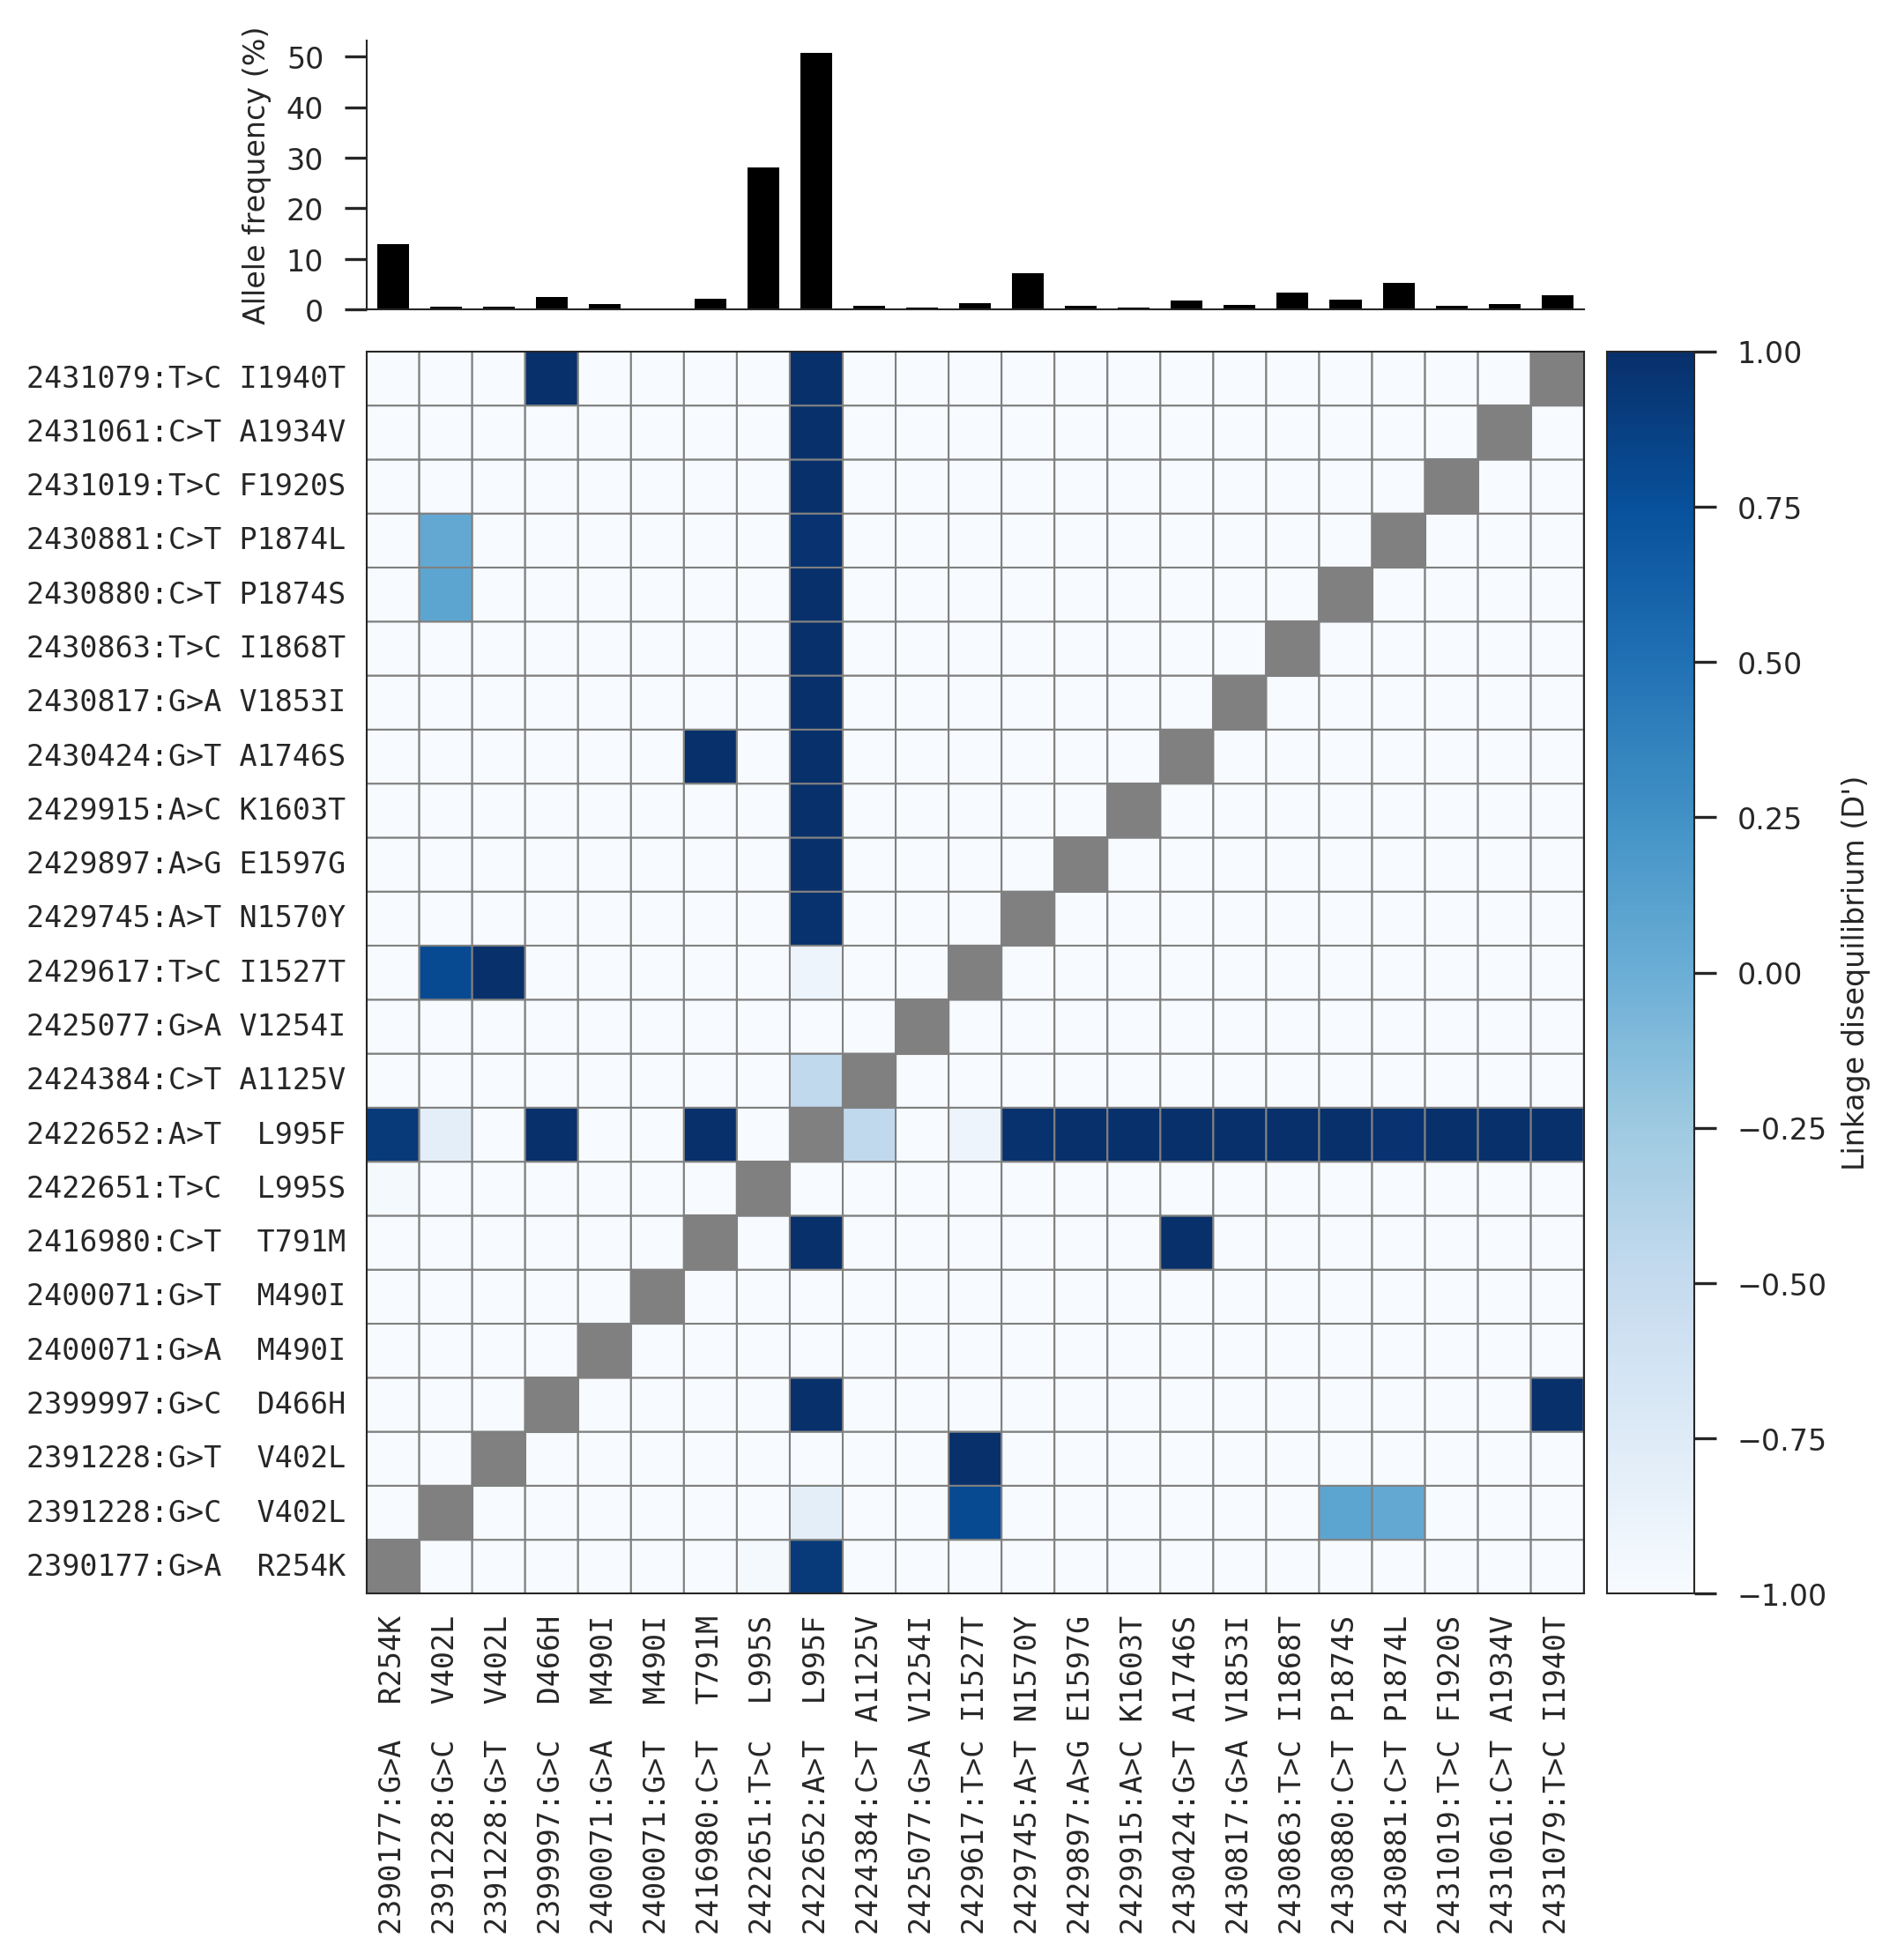
\includegraphics[width=\linewidth]{artwork/fig_ld.png}
  
  \caption{\textbf{Linkage disequilibrium between non-synonymous variants}. A value of 1 indicates that the two variants always occur in combination, and conversely a value of -1 indicates that the two variants never occur in combination. @TODO nuance this?}
  
  \label{fig:ld}
 
\end{figure}
%%


%% Paragraph 4 - L995F enhancers.
%
Of the other 16 SNPs, 13 occurred almost exclusively in combination with \texttt{L995F} (Figure \ref{fig:ld}; \cite{Ag1000gConsortium2017}).
%
These include the \texttt{N1570Y} allele, known to enhance pyrethroid resistance in \textit{An. gambiae} in combination with \texttt{L995F} \cite{Jones2012}.
%
These also include two variants in codon 1874 (\texttt{P1874S}, \texttt{P1874L}). \texttt{P1874S} has previously been found in a colony of the crop pest \textit{Plutella xylostella} with a pyrethroid resistance phenotype, but has not been shown to confer resistance experimentally \cite{Sonoda2008}.
%
10 of these variants, including \texttt{N1570Y} and \texttt{P1874S/L}, occur within internal linker domains of the protein, and so fit the model of variants that may enhance or compensate for the driver phenotype by modifying channel gating behaviour \cite{Smith1997, Jones2012}.
%
The remaining 3 variants are within trans-membrane domains, and so may enhance resistance by altering or interacting with the insecticide binding sites on the VGSC \cite{Dong2014}.
%
Because of the tight linkage between these 13 SNPs and the \texttt{L995F} allele, we classify all as putative \texttt{L995F} enhancers, although experimental work is required to confirm a resistance phenotype.
%%


%% Paragraph 5 - Other high frequency variants we think are probably not resistance variants and why.
%
The remaining 3 variants (\texttt{M490I}, \texttt{A1125V}, \texttt{V1254I}) do not occur in combination with any known resistance allele, and do not appear to be associated with haplotypes under selection \cite{Ag1000gConsortium2017}
%
A possible exception is the \texttt{M490I} allele found at 18\% frequency in the Kenyan population, although the fact that this population has experienced a recent population crash makes it difficult to test for evidence of selection at this locus.
%
All 3 variants occur in internal linker domains, and so do not fit the model of a resistance driver, although experimental work is required to rule out a resistance phenotype.
%
%%


%%%%%%%%%%%%%%%%%%%%%%%%%%%%%%%%%%%%%%%%%%%%%%%%%%%%%%%%%%%%%%%%%%%%%%%%%%%%%%%
\subsection*{Haplotype structure}


%
Although it is known that pyrethroid resistance is increasing in prevalence in malaria vector populations across Africa, it has not been clear whether this is being driven by the spread of resistance alleles via gene flow, or by resistance alleles emerging independently in multiple locations, or by some combination of both processes.
%
The Ag1000G data resource provides a potentially rich source of information about the evolutionary and demographic history of insecticide resistance in any given gene, because data are available not only for SNPs in gene coding regions, but also SNPs in introns and flanking intergenic regions, and in neighbouring genes.
%
These additional variants can be used to analyse the genetic backgrounds (haplotypes) on which resistance alleles are found.
%
In sexually reproducing species, DNA sequences are transmitted from parents to progeny in chunks, rearranged via recombination at each generation, and haplotypes convey information about this history of transmission and recombination, especially when haplotypes from many individuals can be compared.
%


%
In our initial analysis of the \textit{Vgsc} (@@REF Ag1000G), we used 1710 biallelic SNPs from within the @@70 kbp \textit{Vgsc} gene (@@N exonic, @@N intronic) to compute the number of SNP differences between all pairs of 1530 haplotypes derived from 765 wild-caught mosquitoes.
%
This genetic distance measurement is a rough proxy for the degree of relatedness between haplotypes, in the sense that two haplotypes with a small number of SNP differences must be closely related and share a common ancestor in the recent past.
%
This measurement cannot be used to directly estimate the time to most recent common ancestor (TMRCA) for any pair of haplotypes, however, because it does not account for the possibility of recombination events within the gene, which is increasingly likely for pairs of haplotypes that are more distantly related.
%
Nevertheless, it provides a useful tool for exploring patterns of similarity and dissimilarity within the data.
%
To visualise these patterns, we used the pairwise genetic distances to perform hierarchical clustering, which groups similar haplotypes together into clusters.
%
We found that haplotypes carrying resistance alleles were grouped into 10 distinct clusters.
%
Five of these clusters carried the \texttt{L995F} allele (labelled F1-F5), and a further five clusters carried \texttt{L995S} (labelled S1-S5).
%
Within each cluster, haplotypes were nearly identical across all 1710 SNPs (spanning @@70 kbp), and therefore each cluster represents a collection of haplotypes with a very recent common ancestor.
%
Within some of these clusters, we found haplotypes from mosquitoes collected from different locations. 
%
Specifically, cluster F1 contained haplotypes from Guinea, Burkina Faso, Cameroon and Angola; clusters @@ each contained haplotypes from Cameroon and Gabon; and cluster @@ contained haplotypes from Uganda and Kenya.
%
The F1 cluster also contained haplotypes from both \textit{An. gambiae} and \textit{An. coluzzii} individuals.
%
If we assume that haplotypes within each cluster share a common ancestor since the introduction of insecticides, which is reasonable given the high degree of similarity, then each of these clusters provides evidence that resistance alleles have been spreading between geographical locations and species via adaptive gene flow.
%
Here we present several new analyses of these haplotype data, to confirm our initial inferences regarding gene flow, and provide further details regarding the origins and movement of resistance alleles.
%


%% Figure - Haplotype networks.
%
\begin{figure}[!b]
  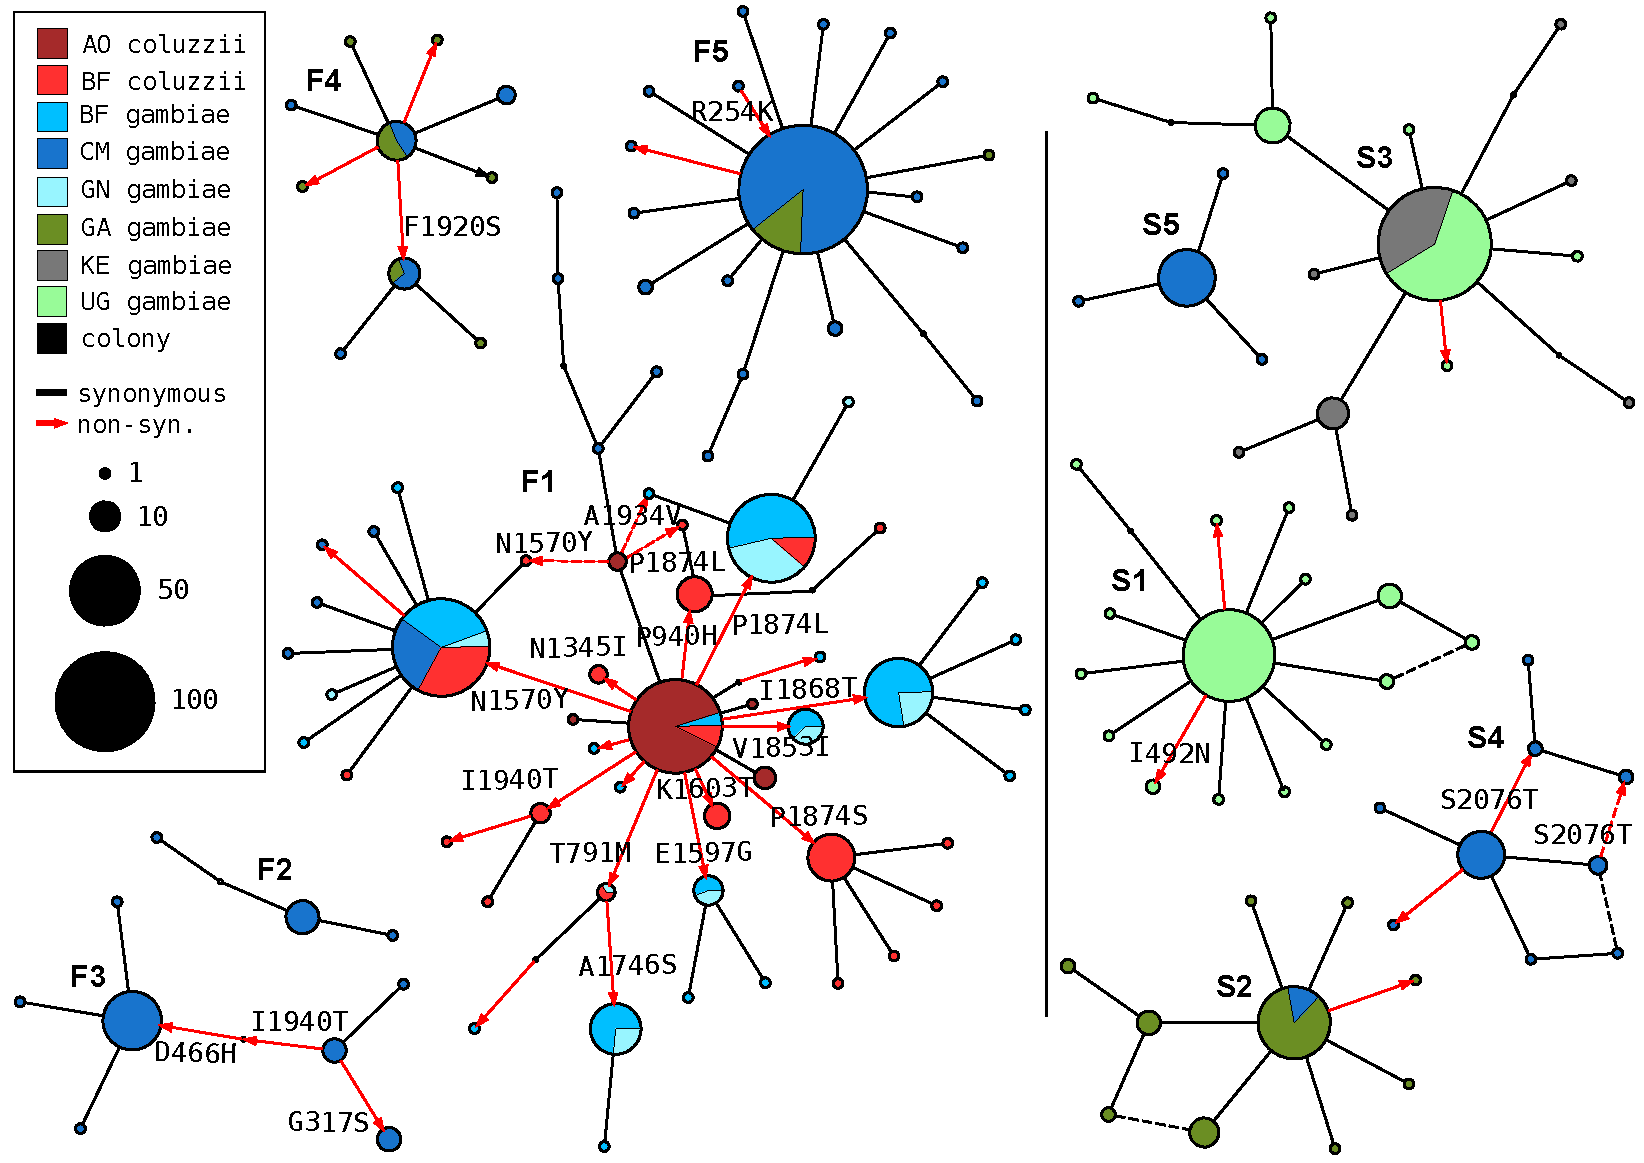
\includegraphics[width=1.1\linewidth,center]{artwork/complete_networks.pdf}
  \caption{\textbf{Haplotype networks}. @@TODO caption}
  \label{fig:networks}
\end{figure}
%%


%% Introduction to the networks.
%
To provide an alternative view of the genetic similarity between haplotypes carrying resistance alleles, we used haplotype data from within the Vgsc gene region to construct median-joining networks (Figure \ref{fig:networks}).
%
This analysis is very similar to hierarchical clustering, except that it allows for the reconstruction and placement of intermediate haplotypes that may not be observed in the data.
%
We constructed these networks up to a maximum distance of @@2 SNP differences, to ensure that each connected component in the resulting networks represents a collection of haplotypes with a recent common ancestor, and thus which is also likely to be minimally affected by recombination within the gene.
%
For haplotypes carrying \texttt{L995F}, the resulting network confirms the presence of five distinct clusters, with close correspondance to the clusters F1-F5 identified previously.
%
The \texttt{L995S} network also confirms five distinct clusters, in concordance with our previous analysis.
%


%% Observations from the networks.
%
The haplotype networks bring into sharp relief the explosive evolution of amino acid substitutions secondary to the \texttt{L995F} allele.
%
Within the F1 network, nodes carrying non-synonymous variants radiate out from a central node carrying only \texttt{L995F}, indicating that the central node represents the ancestral haplotype carrying \texttt{L995F} alone which initially came under selection, and these secondary variants have arisen subsequently as new mutations.
%
Many of the nodes carrying secondary variants are large, consistent with positive selection and a functional role for these secondary variants as enhancers of the \texttt{L995F} resistance phenotype.
%
The F1 network also allows us to infer multiple introgression events between the two species.
%
The central (ancestral) node comprises haplotypes from both species, as do nodes carrying the \texttt{N1570Y}, \texttt{P1874L}, and @@TODO one more variant@@.
%
This structure is consistent with an initial introgression of the ancestral F1 haplotype, followed by introgression of haplotypes carrying secondary mutations.
%
The contrast between the haplotype networks for the \texttt{L995F} and \texttt{L995S} alleles is striking because of the near-total absence of non-synonymous variation within the \texttt{L995S} networks.
%
As we reported previously, this difference is highly significant -- the ratio of non-synonymous to synonymous nucleotide diversity (@@piN/piS) is @@N times higher among haplotypes carrying \texttt{L995F} relative to haplotypes carrying \texttt{L995S} (@@Test; P=@@) (@@REF Ag1000G).
%
Some secondary variants are present within the \texttt{L995S} networks, but all are at low frequency, and thus may be neutral or mildly deleterious variants that are hitch-hiking on selective sweeps for the \texttt{L995S} allele.
%%


%% Limitations of clustering and networks based on genetic distance in a fixed region.
%
While the haplotype clustering and network analyses provide evidence for the spread of resistance alleles via adaptive gene flow, and for the secondary evolution of \texttt{L995F} enhancer alleles, they have several limitations.
%
Within haplotype clusters where gene flow has occurred, they have poor resolution to infer the origin and direction of gene flow.
%
This is because the analyses only leverage information about genetic distance within the \textit{Vgsc} gene, and for very recent events, insufficient time has elapsed for informative mutations to accumulate within this relatively small genome region.
%
Also, the fact that we observe five distinct clusters for each of the codon 995 alleles suggests that each cluster is in some sense independent from the others, and thus gene flow is not required for resistance to emerge in multiple geographical locations.
%
However, the threshold for the genetic distance at which we have chosen to divide haplotypes into different networks or clusters is to a certain extent arbitrary, and based on an intuitive sense of how much variation could have accumulated among the descendants of a single resistant ancestor since the onset of selective pressure.
%
We also need to clarify what we mean by ``independent'', as there are several possible scenarios under which resistance could evolve in multiple populations in the absence of gene flow.
%
Finally, analyses of genetic distance within a fixed genome region can be confounded by recombination events occurring within that region.
%
For example, a recombination event within the \textit{Vgsc} gene upstream of codon 995 could cause us to split a collection of haplotypes into two clusters, even though they are ancestrally related within the region downstream of the recombination event.
%
In the next sub-sections we provide some conceptual foundations to help clarify these ambiguities, and use analyses of haplotype sharing from the genome regions flanking the \textit{Vgsc} gene to provide finer resolution to diagnose recent gene flow events.
%%


%%%%%%%%%%%%%%%%%%%%%%%%%%%%%%%%%%%%%%%%%%%%%%%%%%%%%%%%%%%%%%%%%%%%%%%%%%%%%%%
\subsection*{Recombination}

%%
%
Here we present analyses of recombination both within the \textit{Vgsc} gene itself and on either flank.
%
These provide information about where in the genome recombination events have occurred, and whether these recombination events may have biased or otherwise influenced the outcome of analyses presented in other sections.
%
The analyses also provide information about which haplotypes have experience recent selection, and an alternative view of how different haplotypes are related.
%%


%
EHH analysis first identifies collections of haplotypes with the same alleles at a core locus (@@ref).
%
The haplotypes within each collection are then compared, and the fraction of haplotype pairs that remain identical (EHH) is computed moving both up- and down-stream of the core locus.
%
Recombination events break haplotype homozygosity, and so a slow decay of EHH indicates fewer recombination events, and therefore collections of haplotypes where EHH decays more slowly also provide evidence for positive selection on the core allele.
%
We defined a core region spanning \textit{Vgsc} codon 995 and an additional 4 kbp of flanking sequence (see Methods).
%
Within this core region, we found @@N distinct haplotypes at a frequency > 1\% within the cohort, including core haplotypes representing each of the resistance outbreaks we identified above, and a further @@N core haplotypes not carrying any known or putative resistance allele for comparison.
%
@@TODO finish this
%%

%% Figure - EHH decay
%
\begin{figure}[!b]
  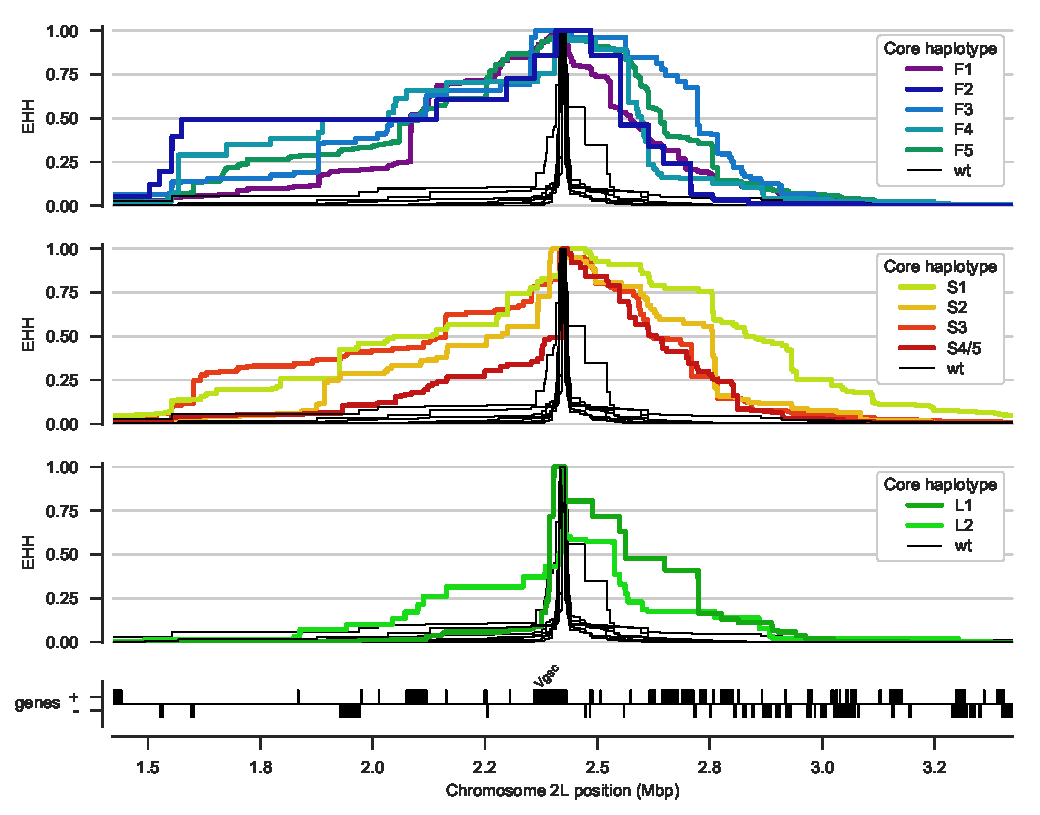
\includegraphics[width=1.1\linewidth,center]{artwork/ehh_decay.pdf}
  \caption{\textbf{EHH decay}. @@TODO caption}
  \label{fig:ehh_decay}
\end{figure}
%%

%%

%%%%%%%%%%%%%%%%%%%%%%%%%%%%%%%%%%%%%%%%%%%%%%%%%%%%%%%%%%%%%%%%%%%%%%%%%%%%%%%
\subsection*{Insecticide resistance outbreaks}


%%
%
To provide an aid to further interpretation of the genetic data, and relating them to the challenges of insecticide resistance management, we introduce the concept of an \textbf{insecticide resistance outbreak}.
%
Informally, we define a resistance outbreak by analogy with the epidemiological concept of an outbreak, as a rapid increase in the prevalence of insecticide resistance among mosquitoes at a particular place and time.
%
Note that this does not imply that the overall abundance of mosquitoes is increase, just that the relative frequency of resistance within mosquito populations is increasing.
%
We also require that all occurrences of insecticide resistance within the same outbreak are connected by a chain of transmission of resistance alleles from parent to progeny mosquitoes, and thus can be traced back to a single resistant common ancestor.
%
A resistance outbreak can be \textbf{localised}, meaning that it affects a small group of mosquitoes of a single species from a limited geographical area.
%
Alternatively, a resistance outbreak may be \textbf{spreading}, meaning that resistance alleles have been transmitted since the introduction of insecticides by interbreeding of mosquitoes of different species and/or originating from different geographical locations.
%
%%


%% Figure - Cartoon of outbreaks.
%
\begin{figure}[!b]
  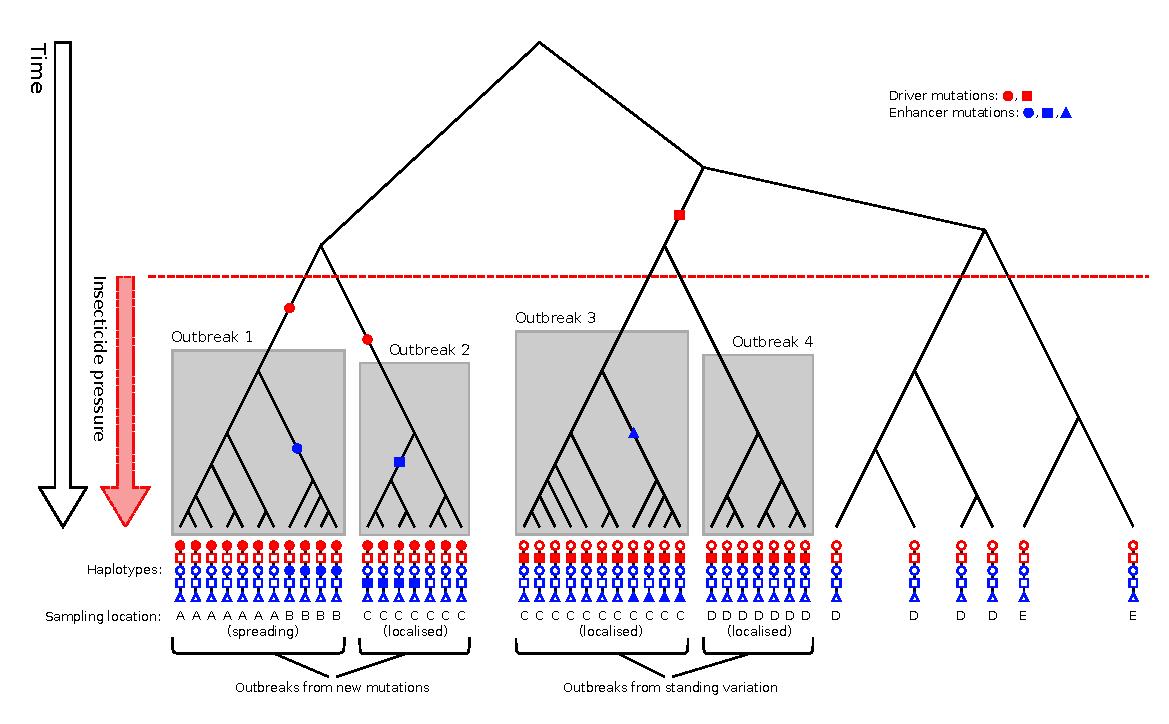
\includegraphics[width=1.1\linewidth,center]{artwork/outbreaks.pdf}
  \caption{\textbf{Illustration of insecticide resistance outbreaks}. @@TODO explanation.}
  \label{fig:outbreaks}
\end{figure}
%%


%%
%
Our goal for the \textit{Vgsc} gene can now be restated, which is to perform an insecticide resistance outbreak analysis.
%
We would like to diagnose how many separate outbreaks have occurred, which outbreaks are localised, and which are spreading.
%
For spreading outbreaks, we would like to reconstruct the path of transmission of resistance alleles between mosquito populations, and to provide information on the probable source. 
%
We would, of course, also like to identify the primary and secondary genetic factors that are driving each outbreak.
%
Stated in this way, it is easier to discuss how this information is potentially relevant to insecticide resistance management, and to frame key epidemiological questions.
%
For example, we would like to begin to build a picture of where and when local conditions have favoured the evolution of insecticide resistance, and whether those conditions are relatively patchy (and hence outbreaks are mainly localised) or whether conditions are consistent over broad areas (and hence can support a spreading outbreak).
%
We would also like to know which mosquito populations are sufficiently connected to enable outbreak spread, and if there is any consistent pattern to the direction of spread.
%
This information could be relevant to discussions about how resources for insecticide resistance management might be targeted, what strategies are appropriate in which settings, and where and when insecticide resistance management needs to be coordinated between different countries and/or at different levels of administration.
%
%%


%%
%
For clarity, we also define the concept of an insecticide resistance outbreak formally in terms of coalescent theory, as a collection of lineages (1) sharing a resistance driver allele by descent, (2) coalescing more recently than the onset of insecticide pressure, and (3) having increased in frequency because of positive selection due to insecticides. 
%
This definition is illustrated for four hypothetical outbreaks in Figure \ref{fig:outbreaks}.
%
Because mosquitoes are sexually recombining, genealogical trees vary along the genome, and so we define resistance outbreaks with respect to a specific gene locus, which for the present study is codon 995 within the \textit{Vgsc} gene.
%
Note that separate outbreaks may be driven by the same resistance allele, and this can occur if multiple mutational events occur after the introduction of insecticides (Figure \ref{fig:outbreaks}, outbreaks 1 and 2), or if a resistance allele is present in mosquito populations as standing variation prior to insecticide use (Figure \ref{fig:outbreaks}, outbreaks 3 and 4).
%
Here we are primarily concerned with whether outbreaks are localised or spreading, because this has immediate epidemiological relevance.
%
We do not attempt to infer whether separate outbreaks with the same driver allele arose via standing variation or new mutations, however this is an interesting biological question to address in future studies.
%
As a technical note, there is a simple correspondance with terminology conventionally used in the population genetics literature to describe selective sweeps.
%
At a given gene locus, a hard selective sweep gives rise to a single resistance outbreak, and a soft selective sweep gives rise to multiple resistance outbreaks.
%%


%%%%%%%%%%%%%%%%%%%%%%%%%%%%%%%%%%%%%%%%%%%%%%%%%%%%%%%%%%%%%%%%%%%%%%%%%%%%%%%
\subsection*{Outbreak analysis from haplotype age}


%% Figure - Overall haplotype age distribution.
%
\begin{figure}[!b]
  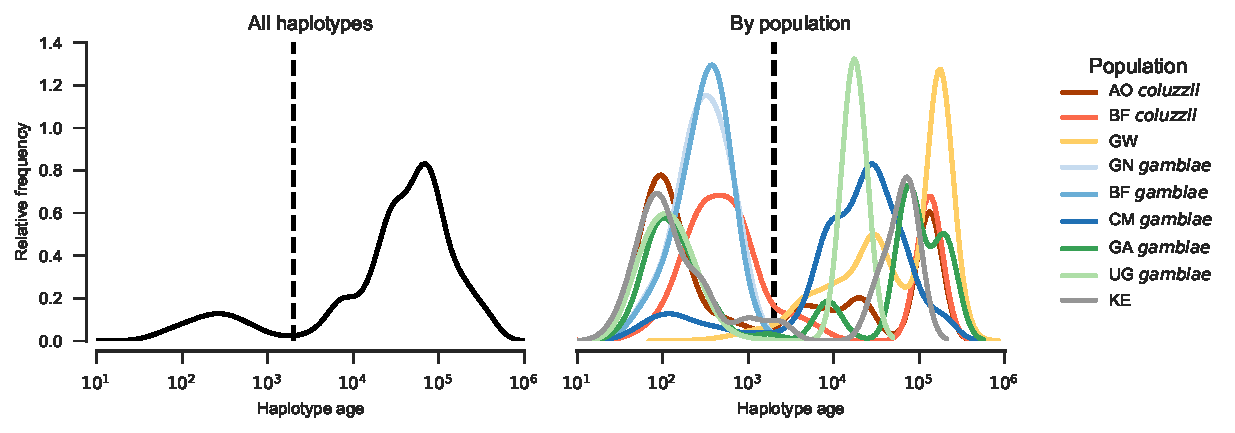
\includegraphics[width=1.1\linewidth,center]{artwork/haplotype_age_dist.pdf}
  \caption{\textbf{Haplotype age distribution}. @@TODO caption.}
  \label{fig:age_hist}
\end{figure}
%%


%%
%
As described above, haplotype data from genome regions both within and flanking the \textit{Vgsc} gene provide a higher resolution for reconstructing recent historical events.
%
To leverage this information, we used a heuristic approach to estimate the time to most recent common ancestor (TMRCA) or ``age'' for each pair of haplotypes in our dataset, centering the analysis on \textit{Vgsc} codon 995.
%
For each pair of haplotypes, we estimated the length of the region shared identical by descent (IBD), and the number of mutations that have accumulated since the most recent common ancestor.
%
We then combined these two pieces of information to produce a point estimate for the haplotype age (Methods).
%
We studied the overall distribution of pairwise haplotype ages (Figure \ref{fig:age_hist}), and used hierarchical clustering to construct a dendrogram and visualise the overall age structure (Figure \ref{fig:tree}).
%
We caution that although the estimated ages are in units of generations, these estimates have not been calibrated, and there is substantial uncertainty regarding both the mutation and recombination rate parameters.
%
The ages therefore should not be interpreted as reliable absolute values, but they can be compared to each other to investigate the relative age of different events.
%%

 
%% Figure - Haplotype age tree.
%
\begin{figure}[!b]
  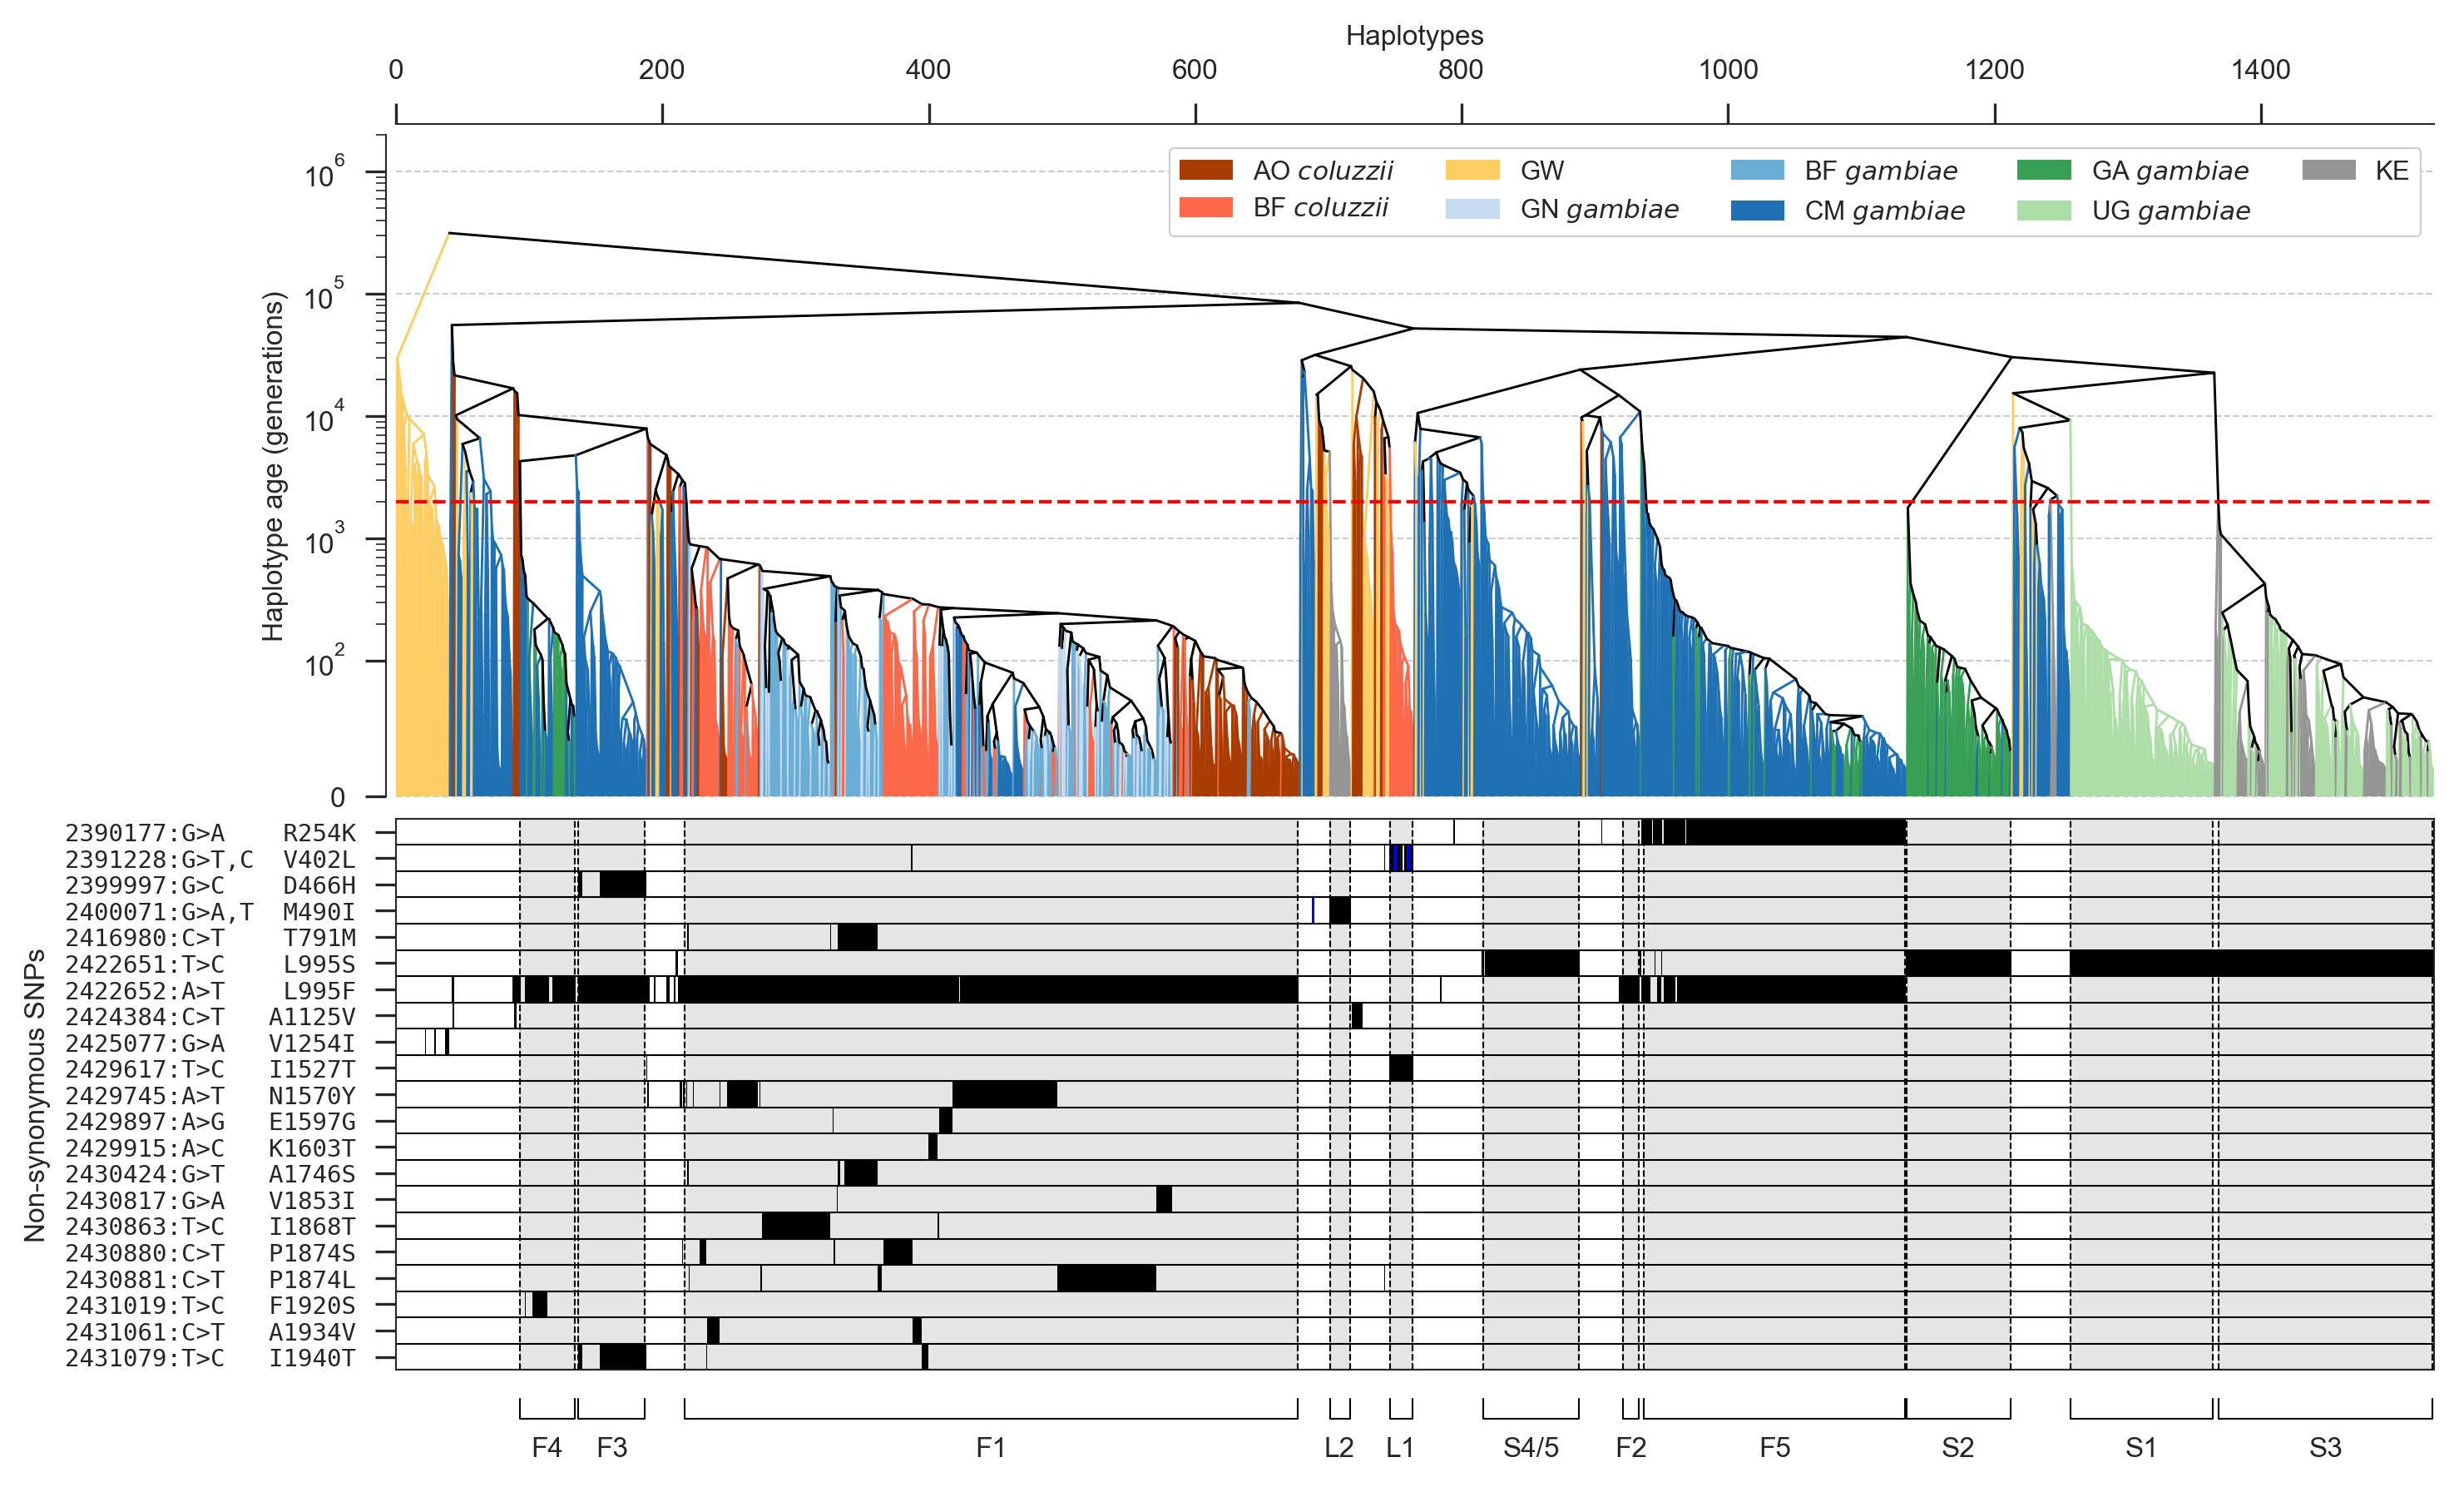
\includegraphics[width=1.1\linewidth,center]{artwork/fig_hap_tree.png}
  \caption{\textbf{Clustering of haplotypes by age}. @@TODO caption.}
  \label{fig:tree}
\end{figure}
%%


%%
%
A key feature of the overall age distribution is that it is bimodal, with a minor mode of haplotypes coalescing recently, and a major mode coalescing further in the past (Figure \ref{fig:age_hist}).
%
This is expected at an insecticide resistance locus experiencing one or more resistance outbreaks.
%
Within each outbreak, all haplotypes share a very recent common ancestor, but between outbreaks and among haplotypes without any resistance allele, haplotypes are more distantly related, and the distribution of ages is influenced by mosquito population size and other demographic factors.
%
In particular, mosquito populations generally have a large effective population size (@@REF Ag1000G), and so in the absence of selection, haplotypes are expected to coalesce slowly.
%
The bimodal age distribution is not due to geographical population structure, because the same bimodality is observed within several populations.
%
We take the midpoint between these two modes as an estimate for the earliest time of onset of selective pressure due to insecticides, and thus for the maximum age of a resistance outbreak.
%
To identify haplotype clusters representing putative resistance outbreaks, we then cut the haplotype dendrogram at this maximum outbreak age (Figure \ref{fig:tree}).
%
Comparing this to previous analyses of haplotype structure based on genetic distance, we find clusters F1-F5 and S1-S3 recapitulated with close correspondence, and S4 and S5 merged into a single cluster.
%
We label a new cluster ``L@@'' representing an outbreak driven by the \texttt{I1527T} allele in combination with one or the other \texttt{V402L} allele.
%
We also label a cluster ``L@@'' capturing a set of haplotypes from Kenya carrying the \texttt{M490I} variant, although the fact that these haplotypes all share a recent common ancestor may be a reflection of the unusual demography of the Kenyan population which has experienced a severe population crash (@@REF) and not be due to recent selection for insecticide resistance.
%
As in earlier analyses, clusters F1, F4, F5 and S3 all include haplotypes sampled from multiple geographical locations, and thus represent spreading outbreaks.
%
Clusters F2, F3, S1, S2, S4/5 and L1 include only haplotypes from a single sampling location, and thus appear to represent localised outbreaks.
%%


%% Figure - Infering spread
%
\begin{figure}[!b]
  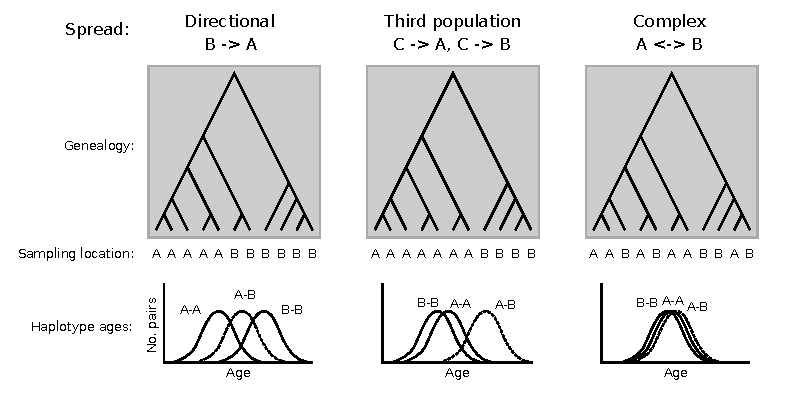
\includegraphics[width=1.1\linewidth,center]{artwork/spreading.pdf}
  \caption{\textbf{Inferring history of spread from haplotype ages}. @@TODO explain.}
  \label{fig:spreading_cartoon}
\end{figure}
%%


%%
%
We then studied the distribution of haplotype ages within each spreading outbreak, to attempt to reconstruct information about the historical path of transmission of resistance alleles between locations.
%
To do this, we grouped the haplotypes within each spreading outbreak by sampling location, and compared the distribution of haplotype ages both within and between locations.
%
To aid in interpreting these data, we define three possible spreading scenarios, being: (1) a directional spread from one population to another; (2) spread from an unsampled population into the sampled populations; and (3) a complex scenario involving multiple gene flow events.
%
In Figure \ref{fig:spreading_cartoon} we illustrate the expected genealogy and haplotype age distribution under each of these scenarios.
%


%%
%
The clearest result was obtained for outbreak F1 (Figure \ref{fig:outbreak_spread}).
%
Within this outbreak, haplotypes from Cameroon and Angola are significantly younger than haplotypes from Burkina Faso and Guinea.
%
The age distributions are consistent with an outbreak originating in West Africa and subsequently spreading towards Cameroon and separately towards Angola.
%
We were surprised that the age distributions for \textit{An. gambiae} and \textit{An. coluzzii} from Burkina Faso are very similar, despite the fact that previous studies have shown that introgression has occurred from \textit{An. gambiae} into \textit{An. coluzzii}.
%
This may indicate that the initial introgression event happened during the early phases of the outbreak, but is also consistent with a complex history of multiple gene flow events between the species.
%%


%% Figure - Age distributions within haplogroups. 
%
\begin{figure}[!b]
  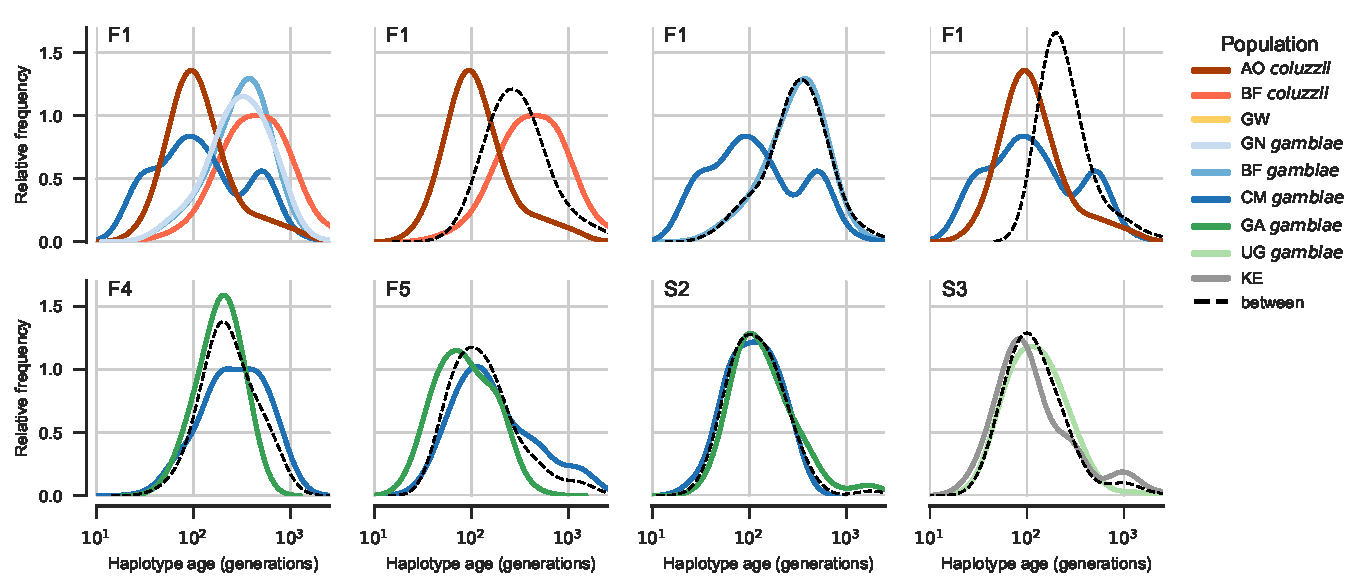
\includegraphics[width=1.1\linewidth,center]{artwork/outbreak_hap_age_dist_3.pdf}
  \caption{\textbf{Haplotype age distributions within spreading outbreaks}. @@TODO caption.}
  \label{fig:outbreak_spread}
\end{figure}
%%


%%
%
Outbreaks F4, F5 and S2 each involve haplotypes from both Cameroon and Gabon.
%
Interpreting the age distributions for these outbreaks is difficult, because mosquitoes from Gabon were collected at a much earlier time point (2000) than mosquitoes from Cameroon (20@@).
%
If our haplotype age estimates were well-calibrated, and we also had reliable estimates for the number of mosquito generations per year, then we might be able to adjust for this time difference, however we are not able to do so presently.
%
An interesting feature of these outbreaks, however, is that we would expect haplotypes from Gabon to appear older due to the time of sampling, which is observed for outbreak S2 but not for F4 or F5.
%
Indeed, S2 is at a high frequency among all Gabon haplotypes and a low frequency among Cameroon haplotypes, whereas the reverse is true for F4 and F5.
%
These data suggest that F4 and F5 have spread from Cameroon towards Gabon, while S2 has spread in the opposite direction.
%
A lot can happen in mosquito populations in @@N years, however, and these conclusions remain highly speculative pending further sampling from both locations. 
%
%%


%%
%
For outbreak S3 involving haplotypes from Uganda and Kenya, the age distributions do not suggest any clear direction of gene flow.
%
This could reflect multiple gene flow events in either or both directions.
%
However, another outbreak (S1) is localised in Uganda and represented within the Ugandan population at roughly equal frequency with S3.
%
If transmission was occurring from Uganda towards Kenya, we might expect both outbreaks to have spread to Kenya.
%
Thus the localisation of S1 suggests S3 has spread into Uganda from Kenya or another location.
%
Again, this conclusion remains tentative and requires confirmation via further sampling.
%%


%% Figure - Map of haplotypes and spread.
%
\begin{figure}[!b]
  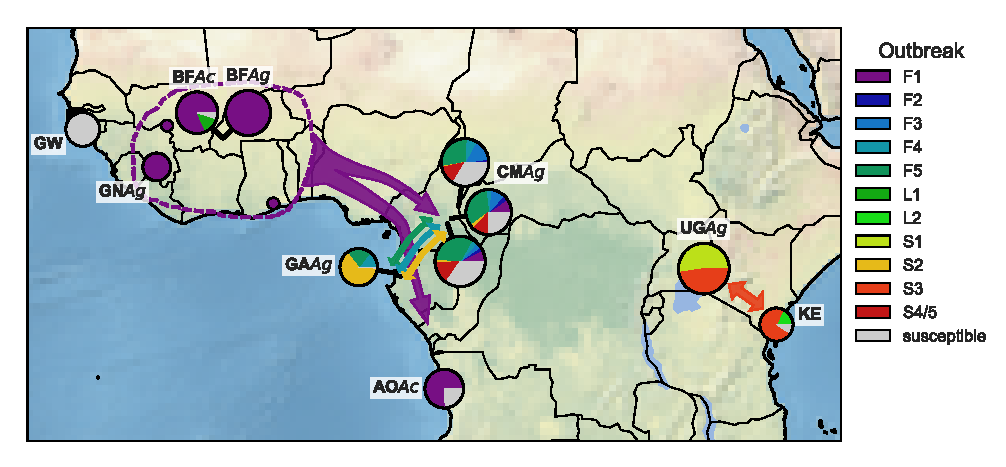
\includegraphics[width=1.1\linewidth,center]{artwork/outbreak_map_edited.pdf}
  \caption{\textbf{Geographical distribution of resistance outbreaks}. @@TODO caption. @@TODO explain Clarkon and Norris points.}
  \label{fig:map}
\end{figure}
%%


%%
%
To summarise these conclusions in a concise way, we have depicted the distribution and spread of resistance outbreaks via the map shown in Figure \ref{fig:map}.
%
We have plotted haplotypes from each sampling location as a pie chart.
%
The overall size of each pie chart represents the number of haplotypes sampled, and coloured wedges within each pie represent the frequency of each resistance outbreak within the population.
%
Coloured arrows are used to depict our inferences regarding the transmission paths for spreading outbreaks.
%
Our conclusions regarding direction of spread for outbreaks F4, F5, S2 and S3 are tentative, and we indicate this with a question mark. 
%
Because of the relatively sparse geographical representation within the Ag1000G phase 1 dataset, and the fact that collections were not synchronized but span several years, we cannot be precise about the geographical origins of these resistance outbreaks.
%
Even for outbreak F1 where we have clear evidence of spread from West Africa towards Central and Southern Africa, we have only sampled mosquitoes from Guinea and Burkina Faso, and the true source of the outbreak may not be either of these countries.
%
We indicate this uncertainty regarding the outbreak source as a coloured area with a dashed border.
%
This representation is imperfect, as is our knowledge regarding the sources and transmission paths of these outbreaks, but we hope this depiction may at least serve to stimulate further sampling, analysis and discussion, with the aim of improving our knowledge of resistance outbreaks for \textit{Vgsc} as well as other insecticide resistance genes.
%%


%%%%%%%%%%%%%%%%%%%%%%%%%%%%%%%%%%%%%%%%%%%%%%%%%%%%%%%%%%%%%%%%%%%%%%%%%%%%%%%
\subsection*{Design of genetic assays for outbreak surveillance}


%%
%
The insecticide resistance outbreaks we have identified here are undoubtedly ongoing, affecting many more mosquito populations than we have sampled in Ag1000G phase 1, and continuing to spread.
%
In addition, other outbreaks may be occurring in populations that we have not sampled, or in populations we have sampled but since the sampling date.
%
Whole-genome sequencing of individual mosquitoes clearly provides data of sufficient resolution to identify resistance outbreaks, and could also be used to provide ongoing outbreak surveillance.
%
The cost of whole-genome sequencing continues to fall, with the present cost being approximately 100 GBP to obtain \textasciitilde$30\times$ coverage of an individual \emph{Anopheles} mosquito genome with 150 bp paired-end reads.
%
Mobile sequencing using nanopore technology is also developing rapidly \cite{Jain2016} and may be a realistic prospect for mosquito whole-genome sequencing within a few years.
%
There is an interim period, however, during which it may be more practical to develop targeted genetic assays for outbreak surveillance that could scale to tens of thousands of mosquitoes at low cost.
%
For example, both next-generation and mobile sequencing platforms can be used for amplicon sequencing, where specific genome regions are amplified and sequenced in highly multiplexed libraries \cite{Bybee2011, Murray2015}.
%%


%% Figure - Information gain.
%
\begin{figure}[!b]
  \centering
  
  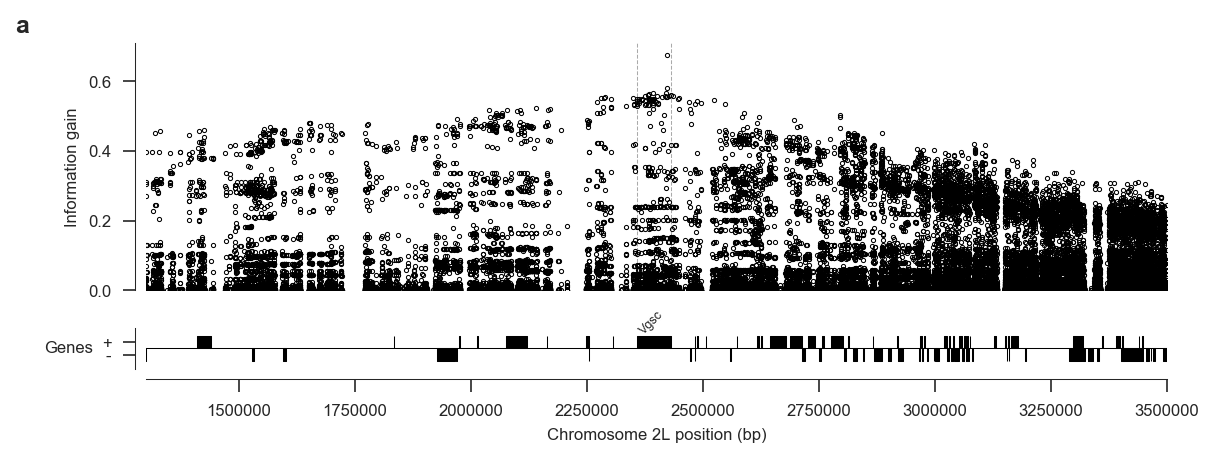
\includegraphics[width=1.0\linewidth]{artwork/info_gain.png}
  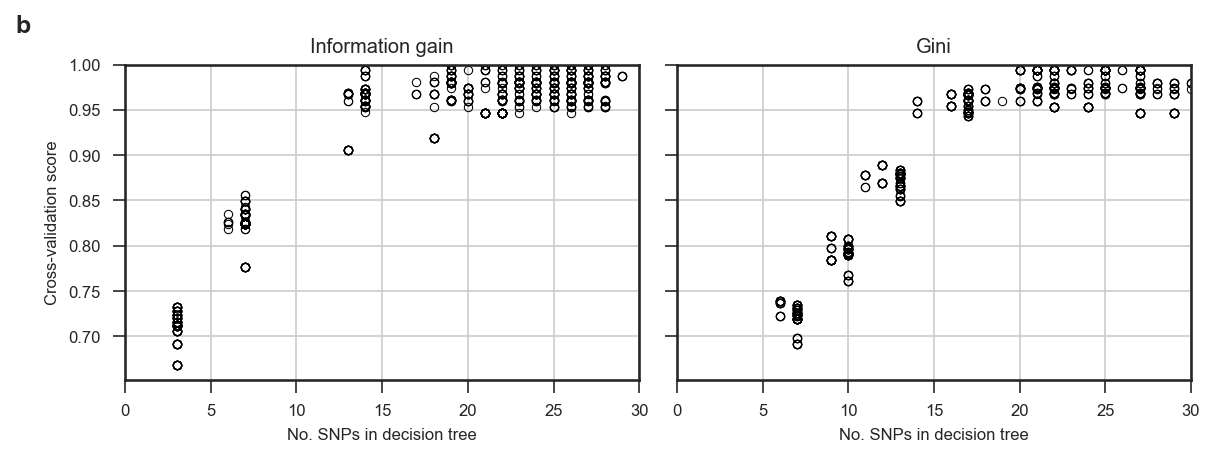
\includegraphics[width=1.0\linewidth]{artwork/tree_cv.png}
  
  \caption{%
%
\textbf{Informative SNPs for outbreak surveillance}. 
%
\textbf{a}, Each data point represents a single SNP. 
%
The information gain value for each SNP provides an indication of how informative the SNP is likely to be if used as part of a genetic assay for testing whether a mosquito carries a resistance haplotype, and if so, which resistance outbreak it derives from. 
%
\textbf{b}, Number of SNPs required to accurately classify which outbreak a haplotype derives from. 
%
Decision trees were constructed using either the LD3 (left) or CART (right) algorithm for comparison.
%
Accuracy was evaluated using 10-fold stratified cross-validation.
}

  \label{fig:gain}
\end{figure}
%%


%%
%
To facilitate the development of targeted genetic assays for \textit{Vgsc} insecticide resistance outbreak surveillance, we have produced two supplementary data tables.
%
In Supplementary Table 1 we provide a list of all biallelic SNPs discovered with high confidence in this study within the \textit{Vgsc} gene and in the 100 kbp upstream and downstream flanking regions.
%
To aid in PCR primer design, for each SNP we provide the flanking sequence for 250 bp upstream and downstream of the SNP position, including information about polymorphisms within these flanking regions.
%
Not all SNPs are informative for detecting whether an individual mosquito carries a haplotype from a resistance outbreak, and we provide some summary statistics for each SNP to aid in the selection of the most informative SNPs.
%
This includes allele frequencies within each of the outbreaks identified here, as well as for populations of susceptible haplotypes.
%
We also provide the overall variance in allele frequencies, the information gain \cite{Quinlan1986}, and the Gini impurity \cite{Breiman1984} for each SNP.
%
Note that recombination events are more likely at increasing distances upstream and downstream of the resistance variants under selection, and thus the most informative SNPs are found closest to the resistance variants within the gene (Figure \ref{fig:gain}).
%
However, SNPs with some information gain are available throughout the gene and in flanking regions.
%


%%
%
We suggest that the design of a genetic assay proceed by (1) performing an initial round of filtering to remove SNPs which are not informative (e.g., low information gain); (2) performing a round of primer design to remove SNPs for which primers are unlikely to be successful; (3) performing a full analysis of the remaining SNPs to select a subset that is sufficient to classify all outbreaks identified here, including some redundancy; (4) finalise primer designs for the chosen panel of SNPs.
%
A possible methodology for step 3 would be to use an algorithm such as ID3 \cite{Quinlan1986} or CART \cite{Breiman1984} to build a decision tree, although many other algorithms for building classifiers are also applicable.
%
To aid in the development of a classifier, in Supplementary Table 2 we provide our classification for each of the 1530 haplotypes sampled here, along with the alleles carried by each haplotype for each of the SNPs included in Supplementary Table 1.
%
To test the methodology, we constructed decision trees using either LD3 or CART algorithms, and using all available SNPs from within the \textit{Vgsc} plus 20 kbp flanking regions as input features (i.e., assuming primers could be designed in all cases).
%
Figure \ref{fig:gain}b shows the cross-validation scores obtained for trees constructed allowing increasing numbers of SNPs.
%
This analysis suggests that it should be possible to construct a tree able to classify haplotypes from all 10 resistance outbreaks with >95\% accuracy using 20 SNPs or less.
%%


%%%%%%%%%%%%%%%%%%%%%%%%%%%%%%%%%%%%%%%%%%%%%%%%%%%%%%%%%%%%%%%%%%%%%%%%%%%%%%%
\subsection*{Recombination}


%%
To look for evidence that haplotypes have experienced recent positive selection, we performed an analysis of extended haplotype homozygosity (EHH) decay @@REF.
%
We defined a core region spanning \textit{Vgsc} codon 995 and an additional 4 kbp of flanking sequence (Methods).
%
Within this core region, we found @@N distinct haplotypes at a frequency > 1\% within the cohort, including core haplotypes representing each of the resistance outbreaks we identified above, and a further @@N core haplotypes not carrying any known or putative resistance allele for comparison.
%
@@TODO finish this
%%

%% Figure - EHH decay
%
\begin{figure}[!b]
  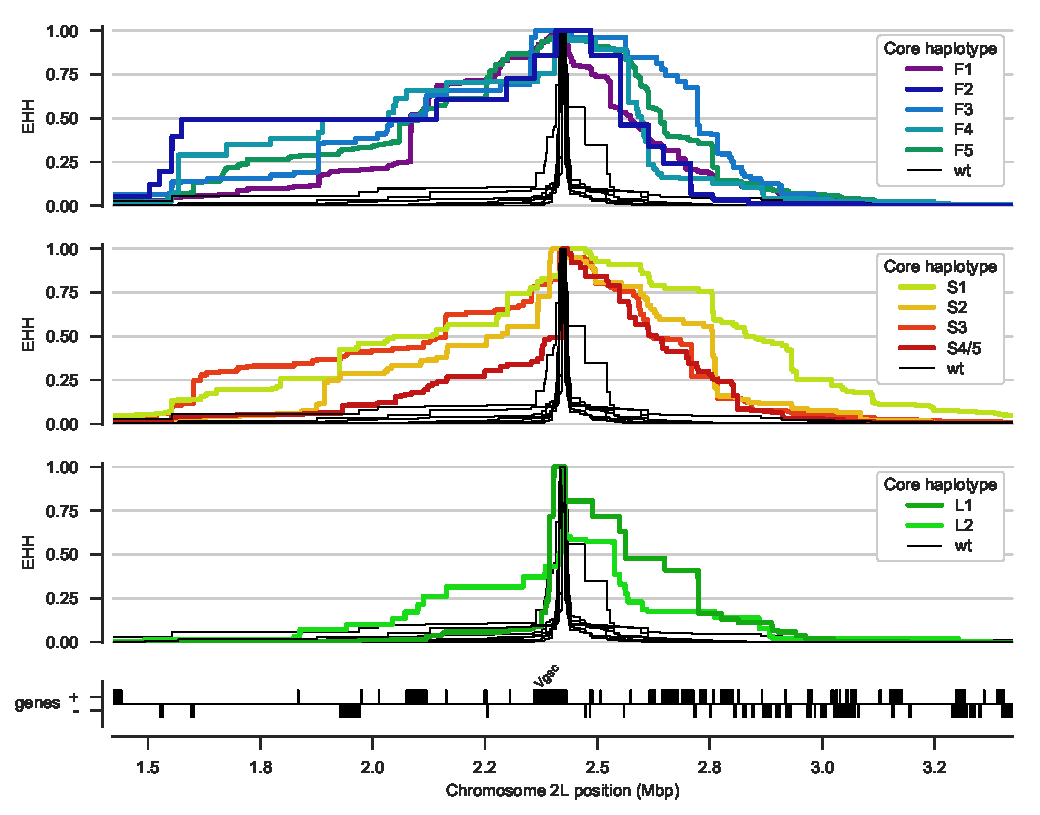
\includegraphics[width=1.1\linewidth,center]{artwork/ehh_decay.pdf}
  \caption{\textbf{EHH decay}. @@TODO caption}
  \label{fig:ehh_decay}
\end{figure}
%%


%%
\textbf{Sandbox paragraph: @@TODO integrate or remove}
%
In this section we present analyses of recombination both within the \textit{Vgsc} gene itself and on either flank.
%
These analyses provide information about which haplotypes have experience recent selection, and an alternative view of how different haplotypes are related.
%
They also provide information about where in the genome recombination events have occurred, and whether these recombination events may have biased or otherwise influenced the outcome of analyses presented in other sections.
%
EHH analysis first identifies collections of haplotypes with the same alleles at a core locus.
%
The haplotypes within each collection are then compared, and the fraction of haplotype pairs that remain identical (EHH) is computed moving both up- and down-stream of the core locus.
%
Recombination events break haplotype homozygosity, and so a slow decay of EHH indicates fewer recombination events, 
%
A collection of haplotypes where EHH decays more slowly provides evidence for positive selection on the core allele, 
%
Haplotypes that have risen rapidly in frequency due to selection will be younger on average, and thus the length of regions of homozygosity between pairs of haplotypes 
%
These analyses provide confirmation of which haplotypes have experience recent positive selection, as haplotypes that have recently increased in frequency will 
%%


%%
%
As mentioned earlier, analyses of haplotype structure based on genetic distance within the fixed window of the \textit{Vgsc} gene could be affected if recombination events occurred within the gene.
%
Our analyses of haplotype age should be less affected by recombination, because they explicitly take recombination into account, estimating the positions at which recombination events have occurred to interrupt regions shared IBD between pairs of haplotypes.
%
However, these analyses were based on a heuristic method for estimating recombination breakpoints, and there are several potential sources of error.
%
To study the evidence for recombination within the genome region spanning the \textit{Vgsc} gene, and provide some additional confirmation that our inferences regarding insecticide resistance outbreaks have not been affected by recombination or other sources of error, we performed an additional analysis of genetic distance between haplotypes.
%
We first constructed a putative ancestral haplotype for each of the outbreaks we identified, by starting from the codon 995 position and separately moving upstream and downstream, assuming the major allele at each SNP bifurcation point represents the ancestral haplotype.
%
We then computed the genetic distance ($D_{XY}$) between each of our sampled haplotypes and each of the inferred ancestral outbreak haplotypes, computing the distance in @@ overlapping windows of @@ bp across a 2 Mbp region spanning the \textit{Vgsc} gene.
%
The results for outbreaks F1-F5 are plotted in Figure \ref{fig:recom_f}, and outbreaks S1-S4/5 are shown in Figure \ref{fig:recom_s}.
%
In these plots we expect that all haplotypes from a given outbreak should share very close genetic similarity ($D_{XY} \approx 0$) with each other and with the ancestral haplotype for that outbreak within the \textit{Vgsc} gene itself, with an increasing number of haplotypes recombining away from the ancestral outbreak haplotype as we move away from the gene in either the upstream or downstream direction.
%
Conversely, haplotypes from one outbreak should not share any close genetic similarity ($D_{XY} > 0$) with the inferred ancestral haplotype from a different outbreak, either within the \textit{Vgsc} gene or in flanking regions.
%%

%% Figure - L995F recombination
%
\begin{figure}[!b]
  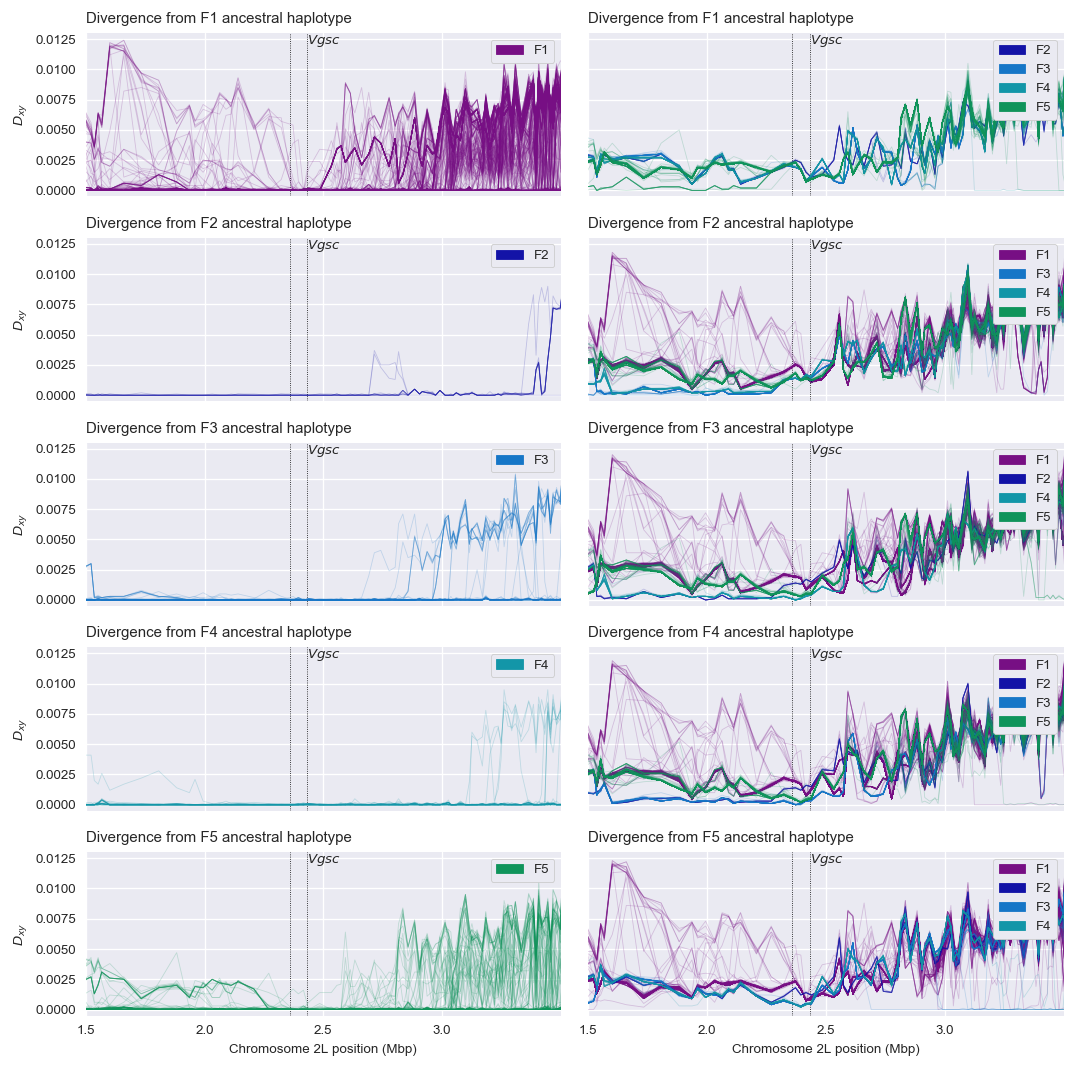
\includegraphics[width=1.1\linewidth,center]{artwork/fig_recom.png}
  \caption{\textbf{Recombination and ancestral haplotypes for L995F}. @@TODO legend}
  \label{fig:recom_f}
\end{figure}
%%


%%
%
The results for all outbreaks are largely consistent with this expectation.
%
For this analysis we treated S4/5 as a single outbreak, as indicated by the haplotype age analysis, and we can gain some insight into why these two were split into separate clusters in earlier analyses.
%
All haplotypes in the S4/5 outbreak share close similarity with the ancestral haplotype on both flanks of the \textit{Vgsc} gene, but there is a short region of within the gene where a subset of haplotypes are diverged.
%
This region of divergence accounts for the S4/S5 split in earlier analyses.
%
@@TODO explain
%
@@TODO also note relatively low divergence among F2, F3, F4 on upstream flank and explain
%%


%%%%%%%%%%%%%%%%%%%%%%%%%%%%%%%%%%%%%%%%%%%%%%%%%%%%%%%%%%%%%%%%%%%%%%%%%%%%%%%
%%%%%%%%%%%%%%%%%%%%%%%%%%%%%%%%%%%%%%%%%%%%%%%%%%%%%%%%%%%%%%%%%%%%%%%%%%%%%%%
\section*{Discussion}


@@TODO Discuss accessibility, have we missed any functional variation?


@@TODO Discuss weaknesses, caveats and potential improvements to method for estimating haplotype age.


@@TODO What are the implications for insecticide resistance management? Realistically how could this information be used?


@@TODO What about DDT? If prior selection for DDT resistance, how might this complicate the picture? Do we see any evidence for multiple phases of selection?


@@TODO Speculate on why \texttt{L995F} but not \texttt{L995S} has evolved secondary variation.


%%%%%%%%%%%%%%%%%%%%%%%%%%%%%%%%%%%%%%%%%%%%%%%%%%%%%%%%%%%%%%%%%%%%%%%%%%%%%%%
%%%%%%%%%%%%%%%%%%%%%%%%%%%%%%%%%%%%%%%%%%%%%%%%%%%%%%%%%%%%%%%%%%%%%%%%%%%%%%%
\section*{Methods}

%%%%%%%%%%%%%%%%%%%%%%%%%%%%%%%%%%%%%%%%%%%%%%%%%%%%%%%%%%%%%%%%%%%%%%%%%%%%%%%
\subsection*{Code}

%
All scripts and Jupyter Notebooks used to generate analyses, figures and tables are available from the GitHub repository \url{https://github.com/malariagen/agam-vgsc-report}. 
%%

%%%%%%%%%%%%%%%%%%%%%%%%%%%%%%%%%%%%%%%%%%%%%%%%%%%%%%%%%%%%%%%%%%%%%%%%%%%%%%%
\subsection*{Data}

%
We used variant call data from the phase 1 AR3 release and phased haplotype data from AR3.1. These data are publically downloadable via ftp from \url{https://www.malariagen.net}. 
%
@@add ENA from paper
%%


%%%%%%%%%%%%%%%%%%%%%%%%%%%%%%%%%%%%%%%%%%%%%%%%%%%%%%%%%%%%%%%%%%%%%%%%%%%%%%%
\subsection*{Data collection and processing}


%
For detailed information on Ag1000g WGS sample collection, sequencing, variant calling, quality control and phasing see \cite{Ag1000gConsortium2017}.
%
In brief, \emph{An. gambiae} and \emph{An. coluzzii} mosquitoes were collected from eight countries across Sub-Saharan Africa: Angola, Burkina Faso, Cameroon, Gabon, Guinea, Guinea Bissau, Kenya and Uganda. 
%
From Angola just \emph{An. coluzzii} were sampled, Burkina Faso had samples of both \emph{An. gambiae} and \emph{An. coluzzii} and all other populations consisted of purely \emph{An. gambiae} except for Kenya and Guinea Bissau, where species status is uncertain \cite{Ag1000gConsortium2017}.
%
Mosquitoes were individually whole genome sequenced on the Illumina HiSeq 2000 platform, generating 100bp paired-end reads. 
%
Sequenced reads were aligned to the \cite{An. gambiae} AgamP3 reference genome assembly \cite{Holt2002}). 
%
Aligned bam files underwent improvement, before variants were called using GATK UnifiedGenotyper. 
%
Quality control included removal of samples with mean coverage <= 14x and an accessibility map was employed following a similar approach to that used for human data by The 1000 Genomes Project Consortium \cite{The1000GenomesProjectConsortium2010}). 
%
Various quality control filters were applied to remove samples and SNPs with poor quality data. 
%
This process produced a call set containing @@n SNPs genotyped in 765 wild-caught individual mosquitoes \cite{Ag1000gConsortium2017}.
%%

%
The Ag1000g variant data was functionally annotated using the SnpEff v4.1b software which allowed investigation of potential phenotype altering variants within \emph{Vgsc} \cite{Cingolani2012}.
%
Non-synonymous \emph{Vgsc} variants were identified as all variants in AGAP004707, 2L:2358158-2431617, with a SnpEff annotation of “missense”  and an ALT allele frequency of >5\% in at least one of the nine mosquito populations, with the exceptions of the multi-allelic SNP 2L:2400071 G>A which is shown despite only being found in \emph{An. gambiae} from Cameroon at 0.4\% frequency, as the G>T variant at the same position which causes the same codon change (\texttt{M490I}), is found above 5\% frequency in Kenya.
%
\texttt{F1920S} is included for continuity with recent \emph{An. gambiae Vgsc} research \cite{Ag1000gConsortium2017}.
%
A minimum ALT allele frequency was employed to discriminate towards variants that may be undergoing selective sweeps and against less informative low frequency alleles.
%%

%
For ease of comparison with previous work on \emph{Vgsc}, pan Insecta, in Table \ref{table:variants_missense} we report codon numbering for both \emph{An. gambiae} and \emph{Musca domestica} (the species in which the gene was first discovered).
%
The \emph{M. domestica Vgsc} sequence (EMBL accession X96668 - \cite{Williamson1996}) was aligned with the \emph{An. gambiae} AGAP004707-RA sequence (AgamP4.4 gene-set), using the Mega v7 software package \cite{Kumar2016}.
%
A map of equivalent codon numbers between the two species can be download from the MalariaGEN website (@@include as supplementary data file?)- 
\url{https://www.malariagen.net/sites/default/files/content/blogs/domestica_gambiae_map.txt}.
%%

%
Haplotypes for each chromosome of each sample were estimated (phased) using using phase informative reads (PIRs) and SHAPEIT2 v2.r837 \cite{Delaneau2013}, see \cite{Ag1000gConsortium2017} supplementary text for more details.
%
The SHAPEIT2 algorithm is unable to phase multi-allelic positions, therefore the two multi-allelic non-synonymous SNPs within the \emph{Vgsc} gene (>5\% ALT frequency in at least one population), altering codons \texttt{V402} and \texttt{M490}, were phased onto the haplotypes using MVNcall v1.0 \cite{Menelaou2013}.
%
Conservative filtering had removed one of the three known insecticide resistance conferring kdr variants, \texttt{N1570Y} \cite{Jones2012}.
%
After manual inspection of the read alignment revealed that the SNP call could be confidently made, it was added back into the data set and then also phased onto the haplotypes using MVNcall.
%
To evaluate the linkage disequilibrium (LD) of non-synonymous \emph{Vgsc} mutations with the two most widespread \emph{kdr} resistance mutations (\texttt{L995S/F}), the D1 statistic was calculated using haplotypes.
%%

%%%%%%%%%%%%%%%%%%%%%%%%%%%%%%%%%%%%%%%%%%%%%%%%%%%%%%%%%%%%%%%%%%%%%%%%%%%%%%%
\subsection*{Haplotype networks}

%
Discerning the relationships between similar haplotypes can be difficult when using bifurcating trees as, inherently, the distance between the leaves at the tips (haplotypes) will be small.
%
As these relationships may be informative of the history of selection, we utilised a network approach to elucidate them.
%
We constructed haplotype networks using the median-joining algorithm \cite{Bandelt1999} as implemented in a custom Python script available from \url{https://github.com/malariagen/agam-vgsc-report}
%
Networks were rendered with the graphviz library and a composite figure constructed using Inkscape.
%%


%%%%%%%%%%%%%%%%%%%%%%%%%%%%%%%%%%%%%%%%%%%%%%%%%%%%%%%%%%%%%%%%%%%%%%%%%%%%%%%
\subsection*{Haplotype age}

%
Haplotype age. @@TODO - AM
-Length of shared haplotype and number of mutations between them are informative of age…
-Pairwise t values were hierarchically clustered and visualised as a dendrogram using the Python library Scipy and its cluster hierarchy functions linkage method.
-Cutting the dendrogram at @@generations clustered haplotypes together into haplogroups…
- Naming of haplogroups with reference to Ag1000g...
-dendro figure/distro figures/map - Python libraries...
%%

%%%%%%%%%%%%%%%%%%%%%%%%%%%%%%%%%%%%%%%%%%%%%%%%%%%%%%%%%%%%%%%%%%%%%%%%%%%%%%%
\subsection*{Recombination}

%
Recombination. @@TODO - AM - Absolute divergence dxy...
%%


%%%%%%%%%%%%%%%%%%%%%%%%%%%%%%%%%%%%%%%%%%%%%%%%%%%%%%%%%%%%%%%%%%%%%%%%%%%%%%%
%%%%%%%%%%%%%%%%%%%%%%%%%%%%%%%%%%%%%%%%%%%%%%%%%%%%%%%%%%%%%%%%%%%%%%%%%%%%%%%
\printbibliography

\end{document}
